\section{Casi d'uso}
\subsection{Introduzione}
In questa sezione del documento vengono analizzati nel dettaglio i casi d'uso individuati in fase di analisi del \href{https://7last.github.io/docs/rtb/documentazione-interna/glossario\#capitolato}{capitolato\textsubscript{G}} e durante i colloqui con la \href{https://7last.github.io/docs/rtb/documentazione-interna/glossario\#proponente}{proponente\textsubscript{G}}.

\subsection{Struttura dei casi d'uso}
In tutto il documento faremo riferimento ai casi d'uso utilizzando la sigla \texttt{UC} seguita dal rispettivo codice nella forma
\begin{center}
	\textbf{UC-[identificativo\_caso\_principale].[identificativo\_sotto\_caso]}
\end{center}
il quale permette di utilizzarlo come riferimento in questo e in altri documenti.\\
Per ciascun caso d'uso vengono definiti i seguenti elementi:
\begin{itemize}
	\item \textbf{attore principale}, entità primariamente coinvolta nel caso d'uso;
	\item \textbf{precondizioni}, le condizioni che devono essere verificate prima che il caso d'uso possa essere eseguito;
	\item \textbf{postcondizioni}, le condizioni che devono essere verificate al termine dell'esecuzione del caso;
	\item \textbf{scenario principale}, la sequenza di passi che descrive il comportamento del sistema durante l'esecuzione del caso d'uso;
	\item \href{https://7last.github.io/docs/rtb/documentazione-interna/glossario\#user-story}{\textbf{user story}\textsubscript{G}}: una descrizione testuale del caso d'uso.
\end{itemize}


\subsection{Attori}
I seguenti attori sono coinvolti nei casi d'uso:
\begin{itemize}
	\item \textbf{autorità locali}, possono accedere al sistema per visualizzare i dati di monitoraggio della \href{https://7last.github.io/docs/rtb/documentazione-interna/glossario\#smart-city}{\textit{Smart City}\textsubscript{G}};
	\item \textbf{sensori}, sorgente di dati con un determinato dominio di interesse che effettua misurazioni e trasmette i dati al sistema.
\end{itemize}

\subsection{Elenco dei casi d'uso}
\subsubsection{UC-1: Visualizzazione dashboard}
\begin{itemize}
	\item \textbf{Attore principale}: autorità locale.
	\item \textbf{Precondizioni}: l'autorità locale ha effettuato l'accesso al sistema ed esso è in funzione.
	\item \textbf{Postcondizioni}: l'autorità locale visualizza la \href{https://7last.github.io/docs/rtb/documentazione-interna/glossario\#dashboard}{dashboard\textsubscript{G}} con i dati relativi ai sensori presenti nella città.
	\item \textbf{Scenario principale}:
	      \begin{enumerate}
		      \item l'autorità locale accede alla piattaforma.
		      \item il sistema carica i dati relativi ai sensori interrogando il database.
	      \end{enumerate}
	\item \href{https://7last.github.io/docs/rtb/documentazione-interna/glossario\#user-story}{\textbf{User story}\textsubscript{G}}:
	      come autorità locale desidero poter visualizzare una \href{https://7last.github.io/docs/rtb/documentazione-interna/glossario\#dashboard}{dashboard\textsubscript{G}} con i dati relativi ai sensori per poter monitorare la loro posizione e i dati trasmessi.
\end{itemize}
\begin{center}
	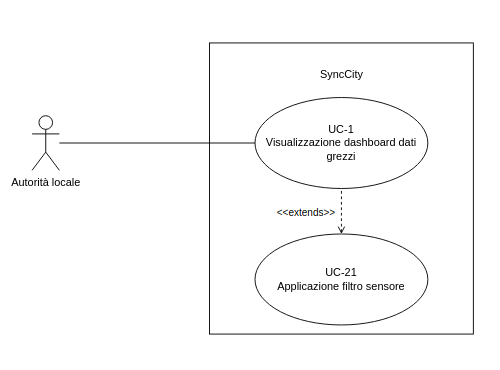
\includegraphics[width=0.6\textwidth]{analisi_dei_requisiti/UC-1.png}
	\captionof{figure}{UC-1: Visualizzazione \href{https://7last.github.io/docs/rtb/documentazione-interna/glossario\#dashboard}{dashboard\textsubscript{G}}}
\end{center}

\subsubsection{UC-2: Visualizzazione dashboard dati grezzi}
\begin{itemize}
	\item \textbf{Attore principale}: autorità locale.
	\item \textbf{Precondizioni}: l'autorità locale ha effettuato l'accesso al sistema ed esso è in funzione.
	\item \textbf{Postcondizioni}: l'autorità locale visualizza la \href{https://7last.github.io/docs/rtb/documentazione-interna/glossario\#dashboard}{dashboard\textsubscript{G}} dei dati grezzi con i dati relativi ai sensori
	      presenti nella città.
	\item \textbf{Scenario principale}:
	      \begin{enumerate}
		      \item l'autorità locale accede alla piattaforma;
		      \item il sistema carica i dati relativi ai sensori interrogando il database.
	      \end{enumerate}
	\item \href{https://7last.github.io/docs/rtb/documentazione-interna/glossario\#user-story}{\textbf{User story}\textsubscript{G}}: come autorità locale desidero poter visualizzare una \href{https://7last.github.io/docs/rtb/documentazione-interna/glossario\#dashboard}{dashboard\textsubscript{G}} dei dati grezzi con i dati relativi ai sensori presenti, la quale mi consente di monitorare quanti e quali sensori sono presenti e la loro posizione.
\end{itemize}
\begin{center}
	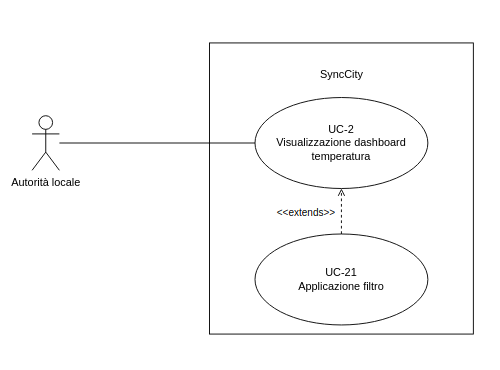
\includegraphics[width=0.6\textwidth]{analisi_dei_requisiti/UC-2.png}
	\captionof{figure}{UC-2: Visualizzazione \href{https://7last.github.io/docs/rtb/documentazione-interna/glossario\#dashboard}{dashboard\textsubscript{G}} dei dati grezzi}
\end{center}

\newpage

\subsubsubsection{UC-2.1: Visualizzazione \textit{panel} con tabella sensori}
\begin{itemize}
	\item \textbf{Attore principale}: autorità locale.
	\item \textbf{Precondizioni}: l'autorità locale ha effettuato l'accesso al sistema ed esso è in funzione.
	\item \textbf{Postcondizioni}: l'autorità locale visualizza il \textit{panel} contenente una tabella di tutti i sensori collegati al sistema.

	\item \textbf{Scenario principale}:
	      \begin{enumerate}
		      \item l'autorità locale accede alla piattaforma;
		      \item il sistema carica i dati relativi ai sensori interrogando il database;
		      \item l'autorità locale seleziona la visualizzazione della \href{https://7last.github.io/docs/rtb/documentazione-interna/glossario\#dashboard}{dashboard\textsubscript{G}} dei dati grezzi.
	      \end{enumerate}
	\item \href{https://7last.github.io/docs/rtb/documentazione-interna/glossario\#user-story}{\textbf{User story}\textsubscript{G}}: come autorità locale desidero poter visualizzare un \textit{panel} contenente una tabella di tutti i sensori collegati al sistema. I dati che devono essere presenti nella tabella sono: identificativo del \href{https://7last.github.io/docs/rtb/documentazione-interna/glossario\#sensore}{sensore\textsubscript{G}}, tipo di \href{https://7last.github.io/docs/rtb/documentazione-interna/glossario\#sensore}{sensore\textsubscript{G}} e data dell'ultima trasmissione. Questi mi consentiranno di avere una visione d'insieme dei sensori presenti.

\end{itemize}
\begin{center}
	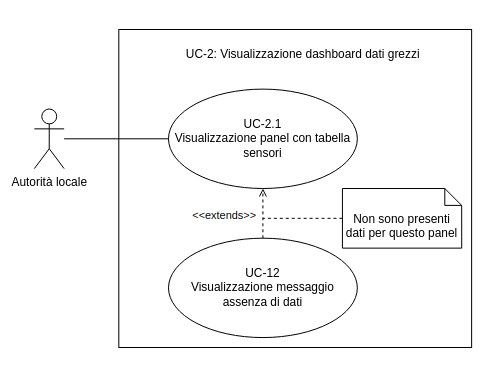
\includegraphics[width=0.6\textwidth]{analisi_dei_requisiti/UC-2.1.png}
	\captionof{figure}{UC-2.1: Visualizzazione \textit{panel} con tabella sensori}
\end{center}

\newpage

\subsubsubsection{UC-2.2: Visualizzazione mappa interattiva sensori}
\begin{itemize}
	\item \textbf{Attore principale}: autorità locale.
	\item \textbf{Precondizioni}: l'autorità locale ha effettuato l'accesso al sistema ed esso è in funzione.
	\item \textbf{Postcondizioni}: l'autorità locale visualizza un \textit{panel} contenente una mappa interattiva
	      popolata con dei marker rappresentanti la posizione dei sensori.
	\item \textbf{Scenario principale}:
	      \begin{enumerate}
		      \item l'autorità locale accede alla piattaforma;
		      \item il sistema carica i dati trasmessi dai sensori interrogando il database;
		      \item l'autorità locale seleziona la visualizzazione della \href{https://7last.github.io/docs/rtb/documentazione-interna/glossario\#dashboard}{dashboard\textsubscript{G}} dei dati grezzi.
	      \end{enumerate}
	\item \href{https://7last.github.io/docs/rtb/documentazione-interna/glossario\#user-story}{\textbf{User story}\textsubscript{G}}: come autorità locale desidero poter visualizzare una mappa interattiva popolata con dei marker rappresentanti
	      la posizione dei sensori e contenenti il loro identificativo. Essa mi consentirà di visualizzare la distribuzione dei sensori nel territorio
	      ed eventualmente di intervenire nel caso in cui siano presenti zone non coperte.
\end{itemize}
\begin{center}
	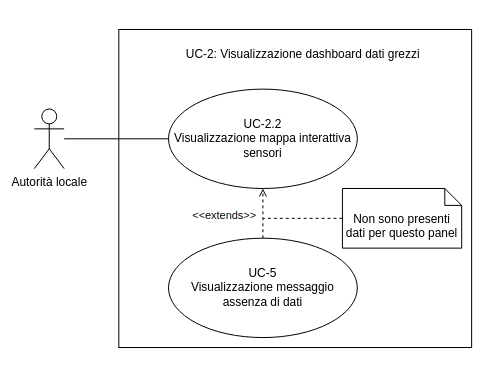
\includegraphics[width=0.6\textwidth]{analisi_dei_requisiti/UC-2.2.png}
	\captionof{figure}{UC-2.2: Visualizzazione mappa interattiva sensori}
\end{center}

\newpage

\subsubsubsection{UC-2.3: Visualizzazione \textit{panel} numero sensori per tipo}
\begin{itemize}
	\item \textbf{Attore principale}: autorità locale.
	\item \textbf{Precondizioni}: l'autorità locale ha effettuato l'accesso al sistema ed esso è in funzione.
	\item \textbf{Postcondizioni}: l'autorità locale visualizza un \textit{panel} contenente il conteggio totale di sensori presenti nel sistema.
	\item \textbf{Scenario principale}:
		\begin{enumerate}
			\item l'autorità locale accede alla piattaforma;
			\item il sistema carica i dati trasmessi dai sensori interrogando il database;
			\item l'autorità locale seleziona la visualizzazione della \href{https://7last.github.io/docs/rtb/documentazione-interna/glossario\#dashboard}{dashboard\textsubscript{G}} dei dati grezzi.
		\end{enumerate}
	\item \href{https://7last.github.io/docs/rtb/documentazione-interna/glossario\#user-story}{\textbf{User story}\textsubscript{G}}:
	      come autorità locale, desidero visualizzare il conteggio totale dei sensori presenti nel sistema, suddivisi per tipologia, per poter valutare l'eventuale necessità di aggiungerne altri.
\end{itemize}
\begin{center}
	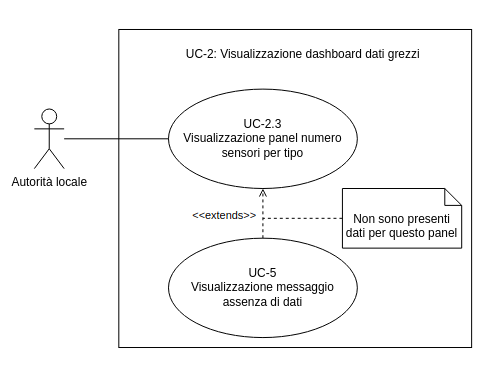
\includegraphics[width=0.6\textwidth]{analisi_dei_requisiti/UC-2.3.png}
	\captionof{figure}{UC-2.3: Visualizzazione \textit{panel} numero sensori per tipo}
\end{center}
\newpage
\subsubsubsection{UC-2.4: Visualizzazione tabella sensori non trasmettenti}
\begin{itemize}
	\item \textbf{Attore principale}: autorità locale.
	\item \textbf{Precondizioni}: l'autorità locale ha effettuato l'accesso al sistema ed esso è in funzione.
	\item \textbf{Postcondizioni}: l'autorità locale visualizza una tabella contenente i sensori che non trasmettono da più di un giorno.
	\item \textbf{Scenario principale}:
	      \begin{enumerate}
		      \item l'autorità locale accede alla piattaforma;
		      \item il sistema carica i dati trasmessi dai sensori interrogando il database;
		      \item l'autorità locale seleziona la visualizzazione della \href{https://7last.github.io/docs/rtb/documentazione-interna/glossario\#dashboard}{dashboard\textsubscript{G}} dei dati grezzi.
	      \end{enumerate}
	\item \href{https://7last.github.io/docs/rtb/documentazione-interna/glossario\#user-story}{\textbf{User story}\textsubscript{G}}:
	      come autorità locale desidero poter visualizzare una tabella contenente i sensori che non trasmettono da più di un giorno, in modo da poter intervenire e ripristinare il corretto funzionamento.
\end{itemize}
\begin{center}
	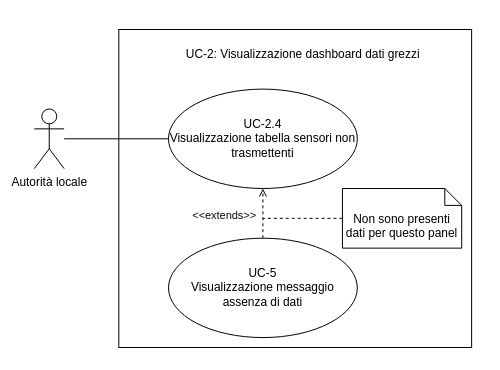
\includegraphics[width=0.6\textwidth]{analisi_dei_requisiti/UC-2.4.png}
	\captionof{figure}{UC-2.4: Visualizzazione tabella sensori che non trasmettono da più di 1 giorno}
\end{center}
\newpage
\subsubsubsection{UC-2.5: Visualizzazione tabella dati grezzi temperatura}
\begin{itemize}
	\item \textbf{Attore principale}: autorità locale.
	\item \textbf{Precondizioni}: l'autorità locale ha effettuato l'accesso al sistema ed esso è in funzione.
	\item \textbf{Postcondizioni}: l'autorità locale visualizza una tabella contenente i dati grezzi trasmessi dai sensori di temperatura.
	\item \textbf{Scenario principale}:
	      \begin{enumerate}
		      \item l'autorità locale accede alla piattaforma;
		      \item il sistema carica i dati trasmessi dai sensori interrogando il database;
		      \item l'autorità locale seleziona la visualizzazione della \href{https://7last.github.io/docs/rtb/documentazione-interna/glossario\#dashboard}{dashboard\textsubscript{G}} dei dati grezzi.
	      \end{enumerate}
	\item \href{https://7last.github.io/docs/rtb/documentazione-interna/glossario\#user-story}{\textbf{User story}\textsubscript{G}}:
	    come autorità locale desidero poter visualizzare una tabella contenente i dati grezzi trasmessi dai sensori di temperatura,
	    in modo da poter analizzare i dati in modo più dettagliato.
\end{itemize}
\begin{center}
	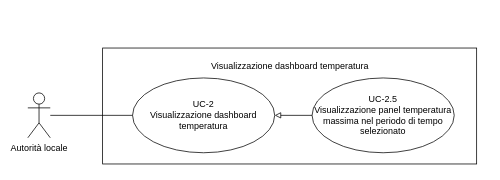
\includegraphics[width=0.6\textwidth]{analisi_dei_requisiti/UC-2.5.png}
	\captionof{figure}{UC-2.5: Visualizzazione tabella dati grezzi temperatura}
\end{center}
\newpage
\subsubsubsection{UC-2.6: Visualizzazione tabella dati grezzi umidità}
\begin{itemize}
	\item \textbf{Attore principale}: autorità locale.
	\item \textbf{Precondizioni}: l'autorità locale ha effettuato l'accesso al sistema ed esso è in funzione.
	\item \textbf{Postcondizioni}: l'autorità locale visualizza una tabella contenente i dati grezzi trasmessi dai sensori di umidità.
	\item \textbf{Scenario principale}:
	      \begin{enumerate}
		      \item l'autorità locale accede alla piattaforma;
		      \item il sistema carica i dati trasmessi dai sensori interrogando il database;
		      \item l'autorità locale seleziona la visualizzazione della \href{https://7last.github.io/docs/rtb/documentazione-interna/glossario\#dashboard}{dashboard\textsubscript{G}} dei dati grezzi.
	      \end{enumerate}
	\item \href{https://7last.github.io/docs/rtb/documentazione-interna/glossario\#user-story}{\textbf{User story}\textsubscript{G}}:
	      come autorità locale desidero poter visualizzare una tabella contenente i dati grezzi trasmessi dai sensori di umidità,
	      in modo da poter analizzare i dati in modo più dettagliato.
\end{itemize}
\begin{center}
	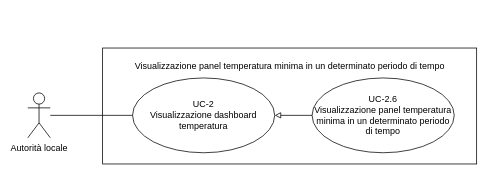
\includegraphics[width=0.6\textwidth]{analisi_dei_requisiti/UC-2.6.png}
	\captionof{figure}{UC-2.6: Visualizzazione tabella dati grezzi umidità}
\end{center}
\newpage
\subsubsubsection{UC-2.7: Visualizzazione tabella dati grezzi traffico}
\begin{itemize}
	\item \textbf{Attore principale}: autorità locale.
	\item \textbf{Precondizioni}: l'autorità locale ha effettuato l'accesso al sistema ed esso è in funzione.
	\item \textbf{Postcondizioni}: l'autorità locale visualizza una tabella contenente i dati grezzi trasmessi dai sensori di traffico.
	\item \textbf{Scenario principale}:
	      \begin{enumerate}
		      \item l'autorità locale accede alla piattaforma;
		      \item il sistema carica i dati trasmessi dai sensori interrogando il database;
		      \item l'autorità locale seleziona la visualizzazione della \href{https://7last.github.io/docs/rtb/documentazione-interna/glossario\#dashboard}{dashboard\textsubscript{G}} dei dati grezzi.
	      \end{enumerate}
	\item \href{https://7last.github.io/docs/rtb/documentazione-interna/glossario\#user-story}{\textbf{User story}\textsubscript{G}}:
	      come autorità locale desidero poter visualizzare una tabella contenente i dati grezzi trasmessi dai sensori di traffico,
	      in modo da poter analizzare i dati in modo più dettagliato.
\end{itemize}
\begin{center}
	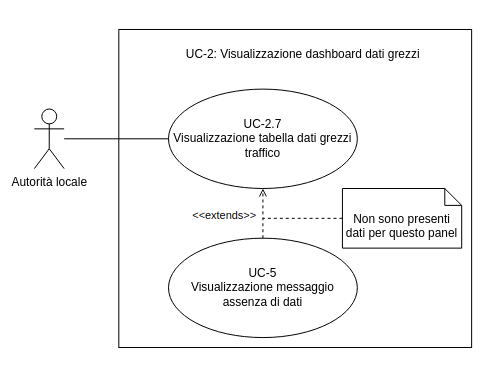
\includegraphics[width=0.6\textwidth]{analisi_dei_requisiti/UC-2.7.png}
	\captionof{figure}{UC-2.7: Visualizzazione tabella dati grezzi traffico}
\end{center}
\newpage
\subsubsubsection{UC-2.8: Visualizzazione tabella dati grezzi qualità dell'aria}
\begin{itemize}
	\item \textbf{Attore principale}: autorità locale.
	\item \textbf{Precondizioni}: l'autorità locale ha effettuato l'accesso al sistema ed esso è in funzione.
	\item \textbf{Postcondizioni}: l'autorità locale visualizza una tabella contenente i dati grezzi trasmessi dai sensori di qualità dell'aria.
	\item \textbf{Scenario principale}:
	      \begin{enumerate}
		      \item l'autorità locale accede alla piattaforma;
		      \item il sistema carica i dati trasmessi dai sensori interrogando il database;
		      \item l'autorità locale seleziona la visualizzazione della \href{https://7last.github.io/docs/rtb/documentazione-interna/glossario\#dashboard}{dashboard\textsubscript{G}} dei dati grezzi.
	      \end{enumerate}
	\item \href{https://7last.github.io/docs/rtb/documentazione-interna/glossario\#user-story}{\textbf{User story}\textsubscript{G}}:
	      come autorità locale desidero poter visualizzare una tabella contenente i dati grezzi trasmessi dai sensori di qualità dell'aria,
	      in modo da poter analizzare i dati in modo più dettagliato.
\end{itemize}
\begin{center}
	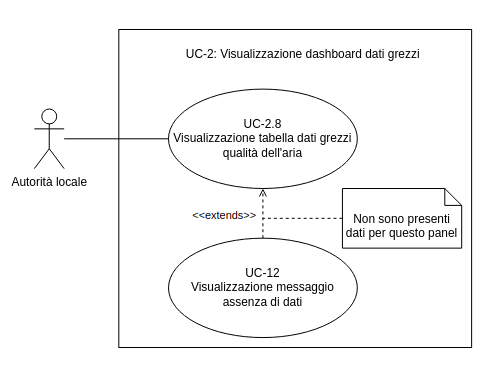
\includegraphics[width=0.6\textwidth]{analisi_dei_requisiti/UC-2.8.png}
	\captionof{figure}{UC-2.8: Visualizzazione tabella dati grezzi qualità dell'aria}
\end{center}

\newpage

\subsubsubsection{UC-2.9: Visualizzazione tabella dati grezzi precipitazioni}
\begin{itemize}
	\item \textbf{Attore principale}: autorità locale.
	\item \textbf{Precondizioni}: l'autorità locale ha effettuato l'accesso al sistema ed esso è in funzione.
	\item \textbf{Postcondizioni}: l'autorità locale visualizza una tabella contenente i dati grezzi trasmessi dai sensori di precipitazioni.
	\item \textbf{Scenario principale}:
	      \begin{enumerate}
		      \item l'autorità locale accede alla piattaforma;
		      \item il sistema carica i dati trasmessi dai sensori interrogando il database;
		      \item l'autorità locale seleziona la visualizzazione della \href{https://7last.github.io/docs/rtb/documentazione-interna/glossario\#dashboard}{dashboard\textsubscript{G}} dei dati grezzi.
	      \end{enumerate}
	\item \href{https://7last.github.io/docs/rtb/documentazione-interna/glossario\#user-story}{\textbf{User story}\textsubscript{G}}:
	      come autorità locale desidero poter visualizzare una tabella contenente i dati grezzi trasmessi dai sensori di precipitazioni,
	      in modo da poter analizzare i dati in modo più dettagliato.
\end{itemize}
\begin{center}
	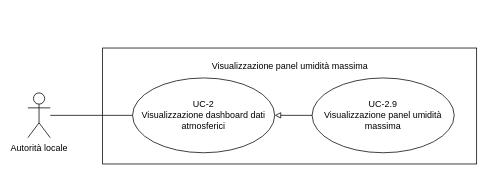
\includegraphics[width=0.6\textwidth]{analisi_dei_requisiti/UC-2.9.png}
	\captionof{figure}{UC-2.9: Visualizzazione tabella dati grezzi precipitazioni}
\end{center}

\newpage

\subsubsubsection{UC-2.10: Visualizzazione tabella dati grezzi isole ecologiche}
\begin{itemize}
	\item \textbf{Attore principale}: autorità locale.
	\item \textbf{Precondizioni}: l'autorità locale ha effettuato l'accesso al sistema ed esso è in funzione.
	\item \textbf{Postcondizioni}: l'autorità locale visualizza una tabella contenente i dati grezzi trasmessi dai sensori di isole ecologiche.
	\item \textbf{Scenario principale}:
	      \begin{enumerate}
		      \item l'autorità locale accede alla piattaforma;
		      \item il sistema carica i dati trasmessi dai sensori interrogando il database;
		      \item l'autorità locale seleziona la visualizzazione della \href{https://7last.github.io/docs/rtb/documentazione-interna/glossario\#dashboard}{dashboard\textsubscript{G}} dei dati grezzi.
	      \end{enumerate}
	\item \href{https://7last.github.io/docs/rtb/documentazione-interna/glossario\#user-story}{\textbf{User story}\textsubscript{G}}:
	      come autorità locale desidero poter visualizzare una tabella contenente i dati grezzi trasmessi dai sensori di isole ecologiche,
	      in modo da poter analizzare i dati in modo più dettagliato.
\end{itemize}
\begin{center}
	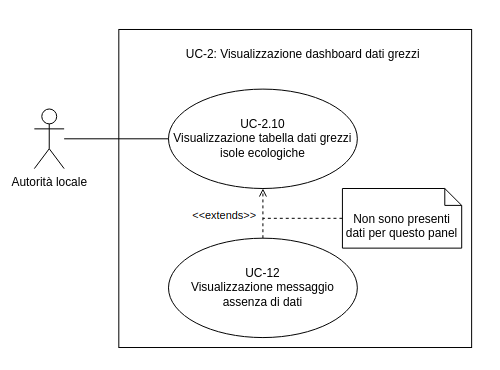
\includegraphics[width=0.6\textwidth]{analisi_dei_requisiti/UC-2.10.png}
	\captionof{figure}{UC-2.10: Visualizzazione tabella dati grezzi isole ecologiche}
\end{center}

\newpage

\subsubsubsection{UC-2.11: Visualizzazione tabella dati grezzi livello di acqua}
\begin{itemize}
	\item \textbf{Attore principale}: autorità locale.
	\item \textbf{Precondizioni}: l'autorità locale ha effettuato l'accesso al sistema ed esso è in funzione.
	\item \textbf{Postcondizioni}: l'autorità locale visualizza una tabella contenente i dati grezzi trasmessi dai sensori di livello di acqua.
	\item \textbf{Scenario principale}:
	      \begin{enumerate}
		      \item l'autorità locale accede alla piattaforma;
		      \item il sistema carica i dati trasmessi dai sensori interrogando il database;
		      \item l'autorità locale seleziona la visualizzazione della \href{https://7last.github.io/docs/rtb/documentazione-interna/glossario\#dashboard}{dashboard\textsubscript{G}} dei dati grezzi.
	      \end{enumerate}
	\item \href{https://7last.github.io/docs/rtb/documentazione-interna/glossario\#user-story}{\textbf{User story}\textsubscript{G}}:
	      come autorità locale desidero poter visualizzare una tabella contenente i dati grezzi trasmessi dai sensori di livello di acqua,
	      in modo da poter analizzare i dati in modo più dettagliato.
\end{itemize}
\begin{center}
	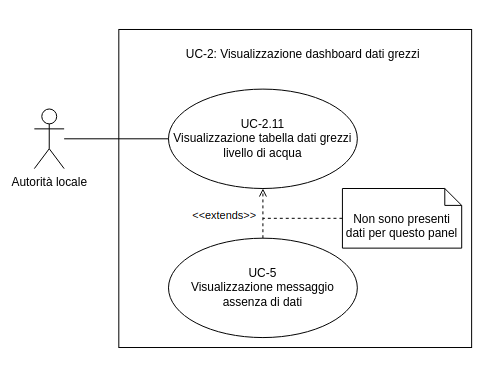
\includegraphics[width=0.6\textwidth]{analisi_dei_requisiti/UC-2.11.png}
	\captionof{figure}{UC-2.11: Visualizzazione tabella dati grezzi livello di acqua}
\end{center}

\newpage

\subsubsubsection{UC-2.12: Visualizzazione tabella dati grezzi colonnine di ricarica}
\begin{itemize}
	\item \textbf{Attore principale}: autorità locale.
	\item \textbf{Precondizioni}: l'autorità locale ha effettuato l'accesso al sistema ed esso è in funzione.
	\item \textbf{Postcondizioni}: l'autorità locale visualizza una tabella contenente i dati grezzi trasmessi dai sensori di colonnine di ricarica.
	\item \textbf{Scenario principale}:
	      \begin{enumerate}
		      \item l'autorità locale accede alla piattaforma;
		      \item il sistema carica i dati trasmessi dai sensori interrogando il database;
		      \item l'autorità locale seleziona la visualizzazione della \href{https://7last.github.io/docs/rtb/documentazione-interna/glossario\#dashboard}{dashboard\textsubscript{G}} dei dati grezzi.
	      \end{enumerate}
	\item \href{https://7last.github.io/docs/rtb/documentazione-interna/glossario\#user-story}{\textbf{User story}\textsubscript{G}}:
	      come autorità locale desidero poter visualizzare una tabella contenente i dati grezzi trasmessi dai sensori di colonnine di ricarica,
	      in modo da poter analizzare i dati in modo più dettagliato.
\end{itemize}
\begin{center}
	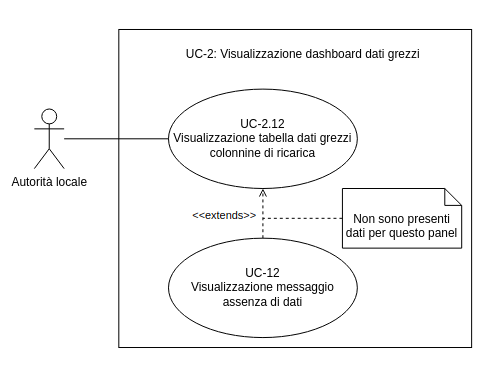
\includegraphics[width=0.6\textwidth]{analisi_dei_requisiti/UC-2.12.png}
	\captionof{figure}{UC-2.12: Visualizzazione tabella dati grezzi colonnine di ricarica}
\end{center}

\newpage

\subsubsubsection{UC-2.13: Visualizzazione grafico time series dati grezzi complessivi temperatura}
\begin{itemize}
	\item \textbf{Attore principale}: autorità locale.
	\item \textbf{Precondizioni}: l'autorità locale ha effettuato l'accesso al sistema ed esso è in funzione.
	\item \textbf{Postcondizioni}: l'autorità locale visualizza un grafico \href{https://7last.github.io/docs/rtb/documentazione-interna/glossario\#time-series}{time series\textsubscript{G}} contenente i dati grezzi trasmessi da tutti i sensori
	      di temperatura presenti nella città.
	\item \textbf{Scenario principale}:
	      \begin{enumerate}
		      \item l'autorità locale accede alla piattaforma;
		      \item il sistema carica i dati trasmessi dai sensori interrogando il database;
		      \item l'autorità locale seleziona la visualizzazione della \href{https://7last.github.io/docs/rtb/documentazione-interna/glossario\#dashboard}{dashboard\textsubscript{G}} dei dati grezzi.
	      \end{enumerate}
	\item \href{https://7last.github.io/docs/rtb/documentazione-interna/glossario\#user-story}{\textbf{User story}\textsubscript{G}}:
	      come autorità locale desidero poter visualizzare un grafico \href{https://7last.github.io/docs/rtb/documentazione-interna/glossario\#time-series}{time series\textsubscript{G}} contenente i dati grezzi trasmessi da tutti i sensori
	      di temperatura presenti nella città, in modo da poterli confrontare tra loro e analizzare in modo più dettagliato.
\end{itemize}
\begin{center}
	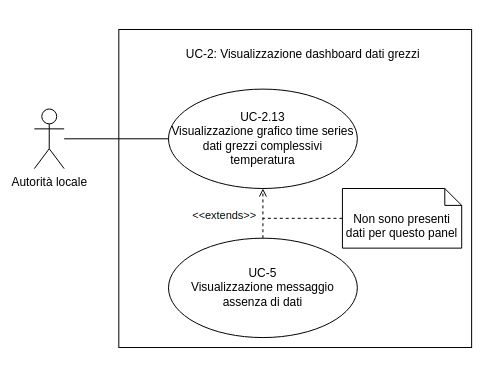
\includegraphics[width=0.6\textwidth]{analisi_dei_requisiti/UC-2.13.png}
	\captionof{figure}{UC-2.6: Visualizzazione grafico \href{https://7last.github.io/docs/rtb/documentazione-interna/glossario\#time-series}{time series\textsubscript{G}} dati grezzi complessivi temperatura}
\end{center}

\newpage

\subsubsubsection{UC-2.14: Visualizzazione grafico time series dati grezzi complessivi umidità}
\begin{itemize}
	\item \textbf{Attore principale}: autorità locale.
	\item \textbf{Precondizioni}: l'autorità locale ha effettuato l'accesso al sistema ed esso è in funzione.
	\item \textbf{Postcondizioni}: l'autorità locale visualizza un grafico \href{https://7last.github.io/docs/rtb/documentazione-interna/glossario\#time-series}{time series\textsubscript{G}} contenente i dati grezzi trasmessi da tutti i sensori
	      di umidità presenti nella città.
	\item \textbf{Scenario principale}:
	      \begin{enumerate}
		      \item l'autorità locale accede alla piattaforma;
		      \item il sistema carica i dati trasmessi dai sensori interrogando il database;
		      \item l'autorità locale seleziona la visualizzazione della \href{https://7last.github.io/docs/rtb/documentazione-interna/glossario\#dashboard}{dashboard\textsubscript{G}} dei dati grezzi.
	      \end{enumerate}
	\item \href{https://7last.github.io/docs/rtb/documentazione-interna/glossario\#user-story}{\textbf{User story}\textsubscript{G}}:
	      come autorità locale desidero poter visualizzare un grafico \href{https://7last.github.io/docs/rtb/documentazione-interna/glossario\#time-series}{time series\textsubscript{G}} contenente i dati grezzi trasmessi da tutti i sensori
	      di umidità presenti nella città, in modo da poterli confrontare tra loro e analizzare in modo più dettagliato.
\end{itemize}
\begin{center}
	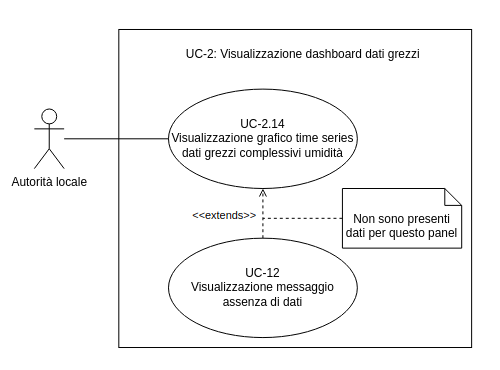
\includegraphics[width=0.6\textwidth]{analisi_dei_requisiti/UC-2.14.png}
	\captionof{figure}{UC-2.14: Visualizzazione grafico \href{https://7last.github.io/docs/rtb/documentazione-interna/glossario\#time-series}{time series\textsubscript{G}} dati grezzi complessivi umidità}
\end{center}

\newpage

\subsubsubsection{UC-2.15: Visualizzazione grafico time series dati grezzi complessivi traffico}
\begin{itemize}
	\item \textbf{Attore principale}: autorità locale.
	\item \textbf{Precondizioni}: l'autorità locale ha effettuato l'accesso al sistema ed esso è in funzione.
	\item \textbf{Postcondizioni}: l'autorità locale visualizza un grafico \href{https://7last.github.io/docs/rtb/documentazione-interna/glossario\#time-series}{time series\textsubscript{G}} contenente i dati grezzi trasmessi da tutti i sensori
	      di traffico presenti nella città.
	\item \textbf{Scenario principale}:
	      \begin{enumerate}
		      \item l'autorità locale accede alla piattaforma;
		      \item il sistema carica i dati trasmessi dai sensori interrogando il database;
		      \item l'autorità locale seleziona la visualizzazione della \href{https://7last.github.io/docs/rtb/documentazione-interna/glossario\#dashboard}{dashboard\textsubscript{G}} dei dati grezzi.
	      \end{enumerate}
	\item \href{https://7last.github.io/docs/rtb/documentazione-interna/glossario\#user-story}{\textbf{User story}\textsubscript{G}}:
	      come autorità locale desidero poter visualizzare un grafico \href{https://7last.github.io/docs/rtb/documentazione-interna/glossario\#time-series}{time series\textsubscript{G}} contenente i dati grezzi trasmessi da tutti i sensori
	      di traffico presenti nella città, in modo da poterli confrontare tra loro e analizzare in modo più dettagliato.
\end{itemize}
\begin{center}
	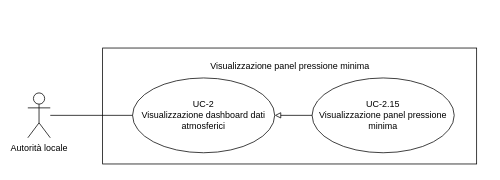
\includegraphics[width=0.6\textwidth]{analisi_dei_requisiti/UC-2.15.png}
	\captionof{figure}{UC-2.15: Visualizzazione grafico \href{https://7last.github.io/docs/rtb/documentazione-interna/glossario\#time-series}{time series\textsubscript{G}} dati grezzi complessivi traffico}
\end{center}

\newpage

\subsubsubsection{UC-2.16: Visualizzazione grafico time series dati grezzi complessivi qualità dell'aria}
\begin{itemize}
	\item \textbf{Attore principale}: autorità locale.
	\item \textbf{Precondizioni}: l'autorità locale ha effettuato l'accesso al sistema ed esso è in funzione.
	\item \textbf{Postcondizioni}: l'autorità locale visualizza un grafico \href{https://7last.github.io/docs/rtb/documentazione-interna/glossario\#time-series}{time series\textsubscript{G}} contenente i dati grezzi trasmessi da tutti i sensori
	      di qualità dell'aria presenti nella città.
	\item \textbf{Scenario principale}:
	      \begin{enumerate}
		      \item l'autorità locale accede alla piattaforma;
		      \item il sistema carica i dati trasmessi dai sensori interrogando il database;
		      \item l'autorità locale seleziona la visualizzazione della \href{https://7last.github.io/docs/rtb/documentazione-interna/glossario\#dashboard}{dashboard\textsubscript{G}} dei dati grezzi.
	      \end{enumerate}
	\item \href{https://7last.github.io/docs/rtb/documentazione-interna/glossario\#user-story}{\textbf{User story}\textsubscript{G}}:
	      come autorità locale desidero poter visualizzare un grafico \href{https://7last.github.io/docs/rtb/documentazione-interna/glossario\#time-series}{time series\textsubscript{G}} contenente i dati grezzi trasmessi da tutti i sensori
	      di qualità dell'aria presenti nella città, in modo da poterli confrontare tra loro e analizzare in modo più dettagliato.
\end{itemize}
\begin{center}
	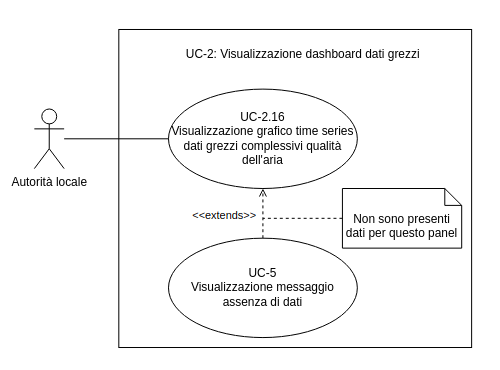
\includegraphics[width=0.6\textwidth]{analisi_dei_requisiti/UC-2.16.png}
	\captionof{figure}{UC-2.16: Visualizzazione grafico \href{https://7last.github.io/docs/rtb/documentazione-interna/glossario\#time-series}{time series\textsubscript{G}} dati grezzi complessivi qualità dell'aria}
\end{center}

\newpage

\subsubsubsection{UC-2.17: Visualizzazione grafico time series dati grezzi complessivi precipitazioni}
\begin{itemize}
	\item \textbf{Attore principale}: autorità locale.
	\item \textbf{Precondizioni}: l'autorità locale ha effettuato l'accesso al sistema ed esso è in funzione.
	\item \textbf{Postcondizioni}: l'autorità locale visualizza un grafico \href{https://7last.github.io/docs/rtb/documentazione-interna/glossario\#time-series}{time series\textsubscript{G}} contenente i dati grezzi trasmessi da tutti i sensori
	      di precipitazioni presenti nella città.
	\item \textbf{Scenario principale}:
	      \begin{enumerate}
		      \item l'autorità locale accede alla piattaforma;
		      \item il sistema carica i dati trasmessi dai sensori interrogando il database;
		      \item l'autorità locale seleziona la visualizzazione della \href{https://7last.github.io/docs/rtb/documentazione-interna/glossario\#dashboard}{dashboard\textsubscript{G}} dei dati grezzi.
	      \end{enumerate}
	\item \href{https://7last.github.io/docs/rtb/documentazione-interna/glossario\#user-story}{\textbf{User story}\textsubscript{G}}:
	      come autorità locale desidero poter visualizzare un grafico \href{https://7last.github.io/docs/rtb/documentazione-interna/glossario\#time-series}{time series\textsubscript{G}} contenente i dati grezzi trasmessi da tutti i sensori
	      di precipitazioni presenti nella città, in modo da poterli confrontare tra loro e analizzare in modo più dettagliato.
\end{itemize}
\begin{center}
	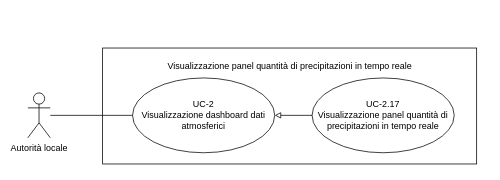
\includegraphics[width=0.6\textwidth]{analisi_dei_requisiti/UC-2.17.png}
	\captionof{figure}{UC-2.17: Visualizzazione grafico \href{https://7last.github.io/docs/rtb/documentazione-interna/glossario\#time-series}{time series\textsubscript{G}} dati grezzi complessivi precipitazioni}
\end{center}

\newpage

\subsubsubsection{UC-2.18: Visualizzazione grafico time series dati grezzi complessivi isole ecologiche}
\begin{itemize}
	\item \textbf{Attore principale}: autorità locale.
	\item \textbf{Precondizioni}: l'autorità locale ha effettuato l'accesso al sistema ed esso è in funzione.
	\item \textbf{Postcondizioni}: l'autorità locale visualizza un grafico \href{https://7last.github.io/docs/rtb/documentazione-interna/glossario\#time-series}{time series\textsubscript{G}} contenente i dati grezzi trasmessi da tutti i sensori
	      di isole ecologiche presenti nella città.
	\item \textbf{Scenario principale}:
	      \begin{enumerate}
		      \item l'autorità locale accede alla piattaforma;
		      \item il sistema carica i dati trasmessi dai sensori interrogando il database;
		      \item l'autorità locale seleziona la visualizzazione della \href{https://7last.github.io/docs/rtb/documentazione-interna/glossario\#dashboard}{dashboard\textsubscript{G}} dei dati grezzi.
	      \end{enumerate}
	\item \href{https://7last.github.io/docs/rtb/documentazione-interna/glossario\#user-story}{\textbf{User story}\textsubscript{G}}:
	      come autorità locale desidero poter visualizzare un grafico \href{https://7last.github.io/docs/rtb/documentazione-interna/glossario\#time-series}{time series\textsubscript{G}} contenente i dati grezzi trasmessi da tutti i sensori
	      di isole ecologiche presenti nella città, in modo da poterli confrontare tra loro e analizzare in modo più dettagliato.
\end{itemize}
\begin{center}
	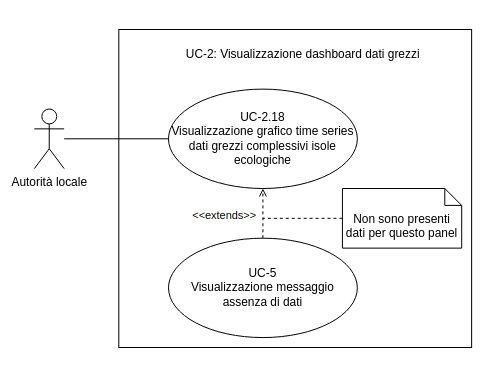
\includegraphics[width=0.6\textwidth]{analisi_dei_requisiti/UC-2.18.png}
	\captionof{figure}{UC-2.18: Visualizzazione grafico \href{https://7last.github.io/docs/rtb/documentazione-interna/glossario\#time-series}{time series\textsubscript{G}} dati grezzi complessivi isole ecologiche}
\end{center}

\newpage

\subsubsubsection{UC-2.19: Visualizzazione grafico time series dati grezzi complessivi livello di acqua}
\begin{itemize}
	\item \textbf{Attore principale}: autorità locale.
	\item \textbf{Precondizioni}: l'autorità locale ha effettuato l'accesso al sistema ed esso è in funzione.
	\item \textbf{Postcondizioni}: l'autorità locale visualizza un grafico \href{https://7last.github.io/docs/rtb/documentazione-interna/glossario\#time-series}{time series\textsubscript{G}} contenente i dati grezzi trasmessi da tutti i sensori
	      di livello di acqua presenti nella città.
	\item \textbf{Scenario principale}:
	      \begin{enumerate}
		      \item l'autorità locale accede alla piattaforma;
		      \item il sistema carica i dati trasmessi dai sensori interrogando il database;
		      \item l'autorità locale seleziona la visualizzazione della \href{https://7last.github.io/docs/rtb/documentazione-interna/glossario\#dashboard}{dashboard\textsubscript{G}} dei dati grezzi.
	      \end{enumerate}
	\item \href{https://7last.github.io/docs/rtb/documentazione-interna/glossario\#user-story}{\textbf{User story}\textsubscript{G}}:
	      come autorità locale desidero poter visualizzare un grafico \href{https://7last.github.io/docs/rtb/documentazione-interna/glossario\#time-series}{time series\textsubscript{G}} contenente i dati grezzi trasmessi da tutti i sensori
	      di livello di acqua presenti nella città, in modo da poterli confrontare tra loro e analizzare in modo più dettagliato.
\end{itemize}
\begin{center}
	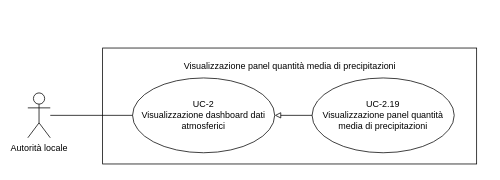
\includegraphics[width=0.6\textwidth]{analisi_dei_requisiti/UC-2.19.png}
	\captionof{figure}{UC-2.19: Visualizzazione grafico \href{https://7last.github.io/docs/rtb/documentazione-interna/glossario\#time-series}{time series\textsubscript{G}} dati grezzi complessivi livello di acqua}
\end{center}

\newpage

\subsubsubsection{UC-2.20: Visualizzazione grafico time series dati grezzi complessivi colonnine di ricarica}
\begin{itemize}
	\item \textbf{Attore principale}: autorità locale.
	\item \textbf{Precondizioni}: l'autorità locale ha effettuato l'accesso al sistema ed esso è in funzione.
	\item \textbf{Postcondizioni}: l'autorità locale visualizza un grafico \href{https://7last.github.io/docs/rtb/documentazione-interna/glossario\#time-series}{time series\textsubscript{G}} contenente i dati grezzi trasmessi da tutti i sensori
	      di colonnine di ricarica presenti nella città.
	\item \textbf{Scenario principale}:
	      \begin{enumerate}
		      \item l'autorità locale accede alla piattaforma;
		      \item il sistema carica i dati trasmessi dai sensori interrogando il database;
		      \item l'autorità locale seleziona la visualizzazione della \href{https://7last.github.io/docs/rtb/documentazione-interna/glossario\#dashboard}{dashboard\textsubscript{G}} dei dati grezzi.
	      \end{enumerate}
	\item \href{https://7last.github.io/docs/rtb/documentazione-interna/glossario\#user-story}{\textbf{User story}\textsubscript{G}}:
	      come autorità locale desidero poter visualizzare un grafico \href{https://7last.github.io/docs/rtb/documentazione-interna/glossario\#time-series}{time series\textsubscript{G}} contenente i dati grezzi trasmessi da tutti i sensori
	      di colonnine di ricarica presenti nella città, in modo da poterli confrontare tra loro e analizzare in modo più dettagliato.
\end{itemize}
\begin{center}
	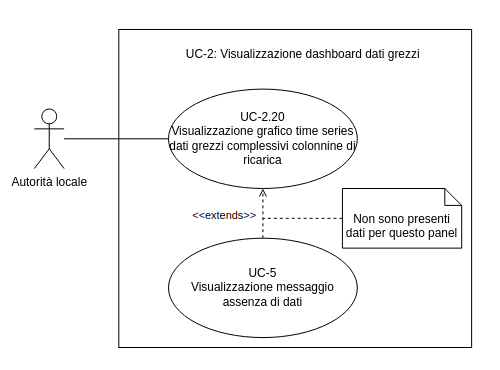
\includegraphics[width=0.6\textwidth]{analisi_dei_requisiti/UC-2.20.png}
	\captionof{figure}{UC-2.20: Visualizzazione grafico \href{https://7last.github.io/docs/rtb/documentazione-interna/glossario\#time-series}{time series\textsubscript{G}} dati grezzi complessivi colonnine di ricarica}
\end{center}

\subsubsection{UC-3: Visualizzazione dashboard temperatura}
\begin{itemize}
	\item \textbf{Attore principale}: autorità locale.
	\item \textbf{Precondizioni}: l'autorità locale ha effettuato l'accesso al sistema ed esso è in funzione.
	\item \textbf{Postcondizioni}: l'autorità locale visualizza la \href{https://7last.github.io/docs/rtb/documentazione-interna/glossario\#dashboard}{dashboard\textsubscript{G}} relativa
	      ai sensori di temperatura presenti nella città.
	\item \textbf{Scenario principale}:
	      \begin{enumerate}
		      \item l'autorità locale accede alla piattaforma;
		      \item il sistema carica i dati trasmessi dai sensori interrogando il database;
		      \item l'autorità locale seleziona la visualizzazione della \href{https://7last.github.io/docs/rtb/documentazione-interna/glossario\#dashboard}{dashboard\textsubscript{G}} relativa ai sensori di temperatura.
	      \end{enumerate}
	\item \href{https://7last.github.io/docs/rtb/documentazione-interna/glossario\#user-story}{\textbf{User story}\textsubscript{G}}:
	      come autorità locale desidero poter visualizzare una \href{https://7last.github.io/docs/rtb/documentazione-interna/glossario\#dashboard}{dashboard\textsubscript{G}} relativa ai sensori di temperatura presenti nella città, la quale
	      dovrà contenere informazioni utili per monitorare l'andamento della temperatura sulla base di dati storici e in tempo reale, mostrando
	      anche statistiche come la temperatura media, massima e minima nel periodo di tempo selezionato.
\end{itemize}
\begin{center}
	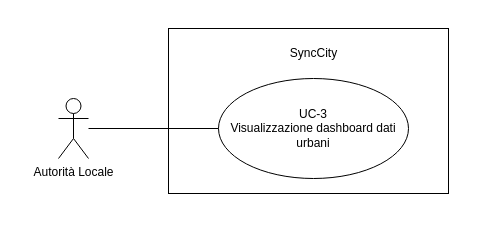
\includegraphics[width=0.6\textwidth]{analisi_dei_requisiti/UC-3.png}
	\captionof{figure}{UC-3: Visualizzazione \href{https://7last.github.io/docs/rtb/documentazione-interna/glossario\#dashboard}{dashboard\textsubscript{G}} temperatura}
\end{center}

\newpage

\subsubsubsection{UC-3.1: Visualizzazione grafico time series temperatura}
\begin{itemize}
	\item \textbf{Attore principale}: autorità locale.
	\item \textbf{Precondizioni}:
	      \begin{enumerate}
		      \item l'autorità locale ha effettuato l'accesso al sistema ed esso è in funzione;
		      \item il sistema ha caricato la \href{https://7last.github.io/docs/rtb/documentazione-interna/glossario\#dashboard}{dashboard\textsubscript{G}} relativa ai sensori di temperatura.
	      \end{enumerate}
	\item \textbf{Postcondizioni}: l'autorità locale visualizza un grafico \href{https://7last.github.io/docs/rtb/documentazione-interna/glossario\#time-series}{time series\textsubscript{G}} contenente le misurazioni storiche
	      della temperatura aggregate per 5 minuti.
	\item \textbf{Scenario principale}:
	      \begin{enumerate}
		      \item l'autorità locale accede alla piattaforma;
		      \item il sistema carica i dati relativi ai sensori interrogando il database;
		      \item l'autorità locale seleziona la visualizzazione della \href{https://7last.github.io/docs/rtb/documentazione-interna/glossario\#dashboard}{dashboard\textsubscript{G}} relativa ai sensori di temperatura.
	      \end{enumerate}
	\item \href{https://7last.github.io/docs/rtb/documentazione-interna/glossario\#user-story}{\textbf{User story}\textsubscript{G}}: come autorità locale desidero poter visualizzare un grafico \href{https://7last.github.io/docs/rtb/documentazione-interna/glossario\#time-series}{time series\textsubscript{G}} contenente le misurazioni storiche della temperatura
	      per poter monitorarne l'andamento nel tempo e facilmente individuare eventuali anomalie.
\end{itemize}
\begin{center}
	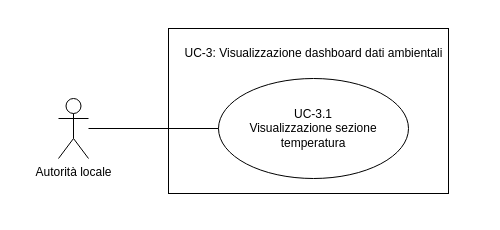
\includegraphics[width=0.70\textwidth]{analisi_dei_requisiti/UC-3.1.png}
	\captionof{figure}{UC-3.1: Visualizzazione grafico \href{https://7last.github.io/docs/rtb/documentazione-interna/glossario\#time-series}{time series\textsubscript{G}} per temperatura}
\end{center}

\newpage

\subsubsubsection{UC-3.2: Visualizzazione mappa sensori temperatura}
\begin{itemize}
	\item \textbf{Attore principale}: autorità locale.
	\item \textbf{Precondizioni}:
	      \begin{enumerate}
		      \item l'autorità locale ha effettuato l'accesso al sistema ed esso è in funzione;
		      \item il sistema ha caricato la \href{https://7last.github.io/docs/rtb/documentazione-interna/glossario\#dashboard}{dashboard\textsubscript{G}} relativa ai sensori di temperatura.
	      \end{enumerate}
	\item \textbf{Postcondizioni}: l'autorità locale visualizza una mappa interattiva popolata con dei marker rappresentanti la posizione dei sensori di temperatura.
	\item \textbf{Scenario principale}:
	      \begin{enumerate}
		      \item l'autorità locale accede alla piattaforma;
		      \item il sistema carica i dati relativi ai sensori interrogando il database;
		      \item l'autorità locale seleziona la visualizzazione della \href{https://7last.github.io/docs/rtb/documentazione-interna/glossario\#dashboard}{dashboard\textsubscript{G}} relativa ai sensori di temperatura.
	      \end{enumerate}
	\item \href{https://7last.github.io/docs/rtb/documentazione-interna/glossario\#user-story}{\textbf{User story}\textsubscript{G}}:
	      come autorità locale desidero poter visualizzare una mappa interattiva popolata con dei marker rappresentanti la posizione dei sensori di temperatura e contenenti il loro identificativo. Essa mi consentirà di visualizzare la distribuzione dei sensori di temperatura nel territorio ed eventualmente intervenire nel caso in cui siano presenti zone non coperte.
\end{itemize}
\begin{center}
	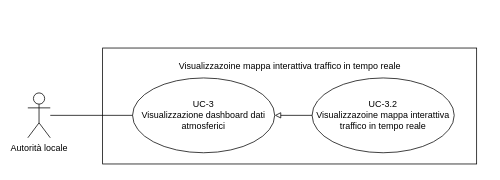
\includegraphics[width=0.62\textwidth]{analisi_dei_requisiti/UC-3.2.png}
	\captionof{figure}{UC-3.2: Visualizzazione mappa interattiva sensori temperatura}
\end{center}

\newpage

\subsubsubsection{UC-3.3: Visualizzazione \textit{panel} temperatura media nel periodo di tempo selezionato}
\begin{itemize}
	\item \textbf{Attore principale}: autorità locale.
	\item \textbf{Precondizioni}:
	      \begin{enumerate}
		      \item l'autorità locale ha effettuato l'accesso al sistema ed esso è in funzione;
		      \item il sistema ha caricato la \href{https://7last.github.io/docs/rtb/documentazione-interna/glossario\#dashboard}{dashboard\textsubscript{G}} relativa ai sensori di temperatura.
	      \end{enumerate}
	\item \textbf{Postcondizioni}: l'autorità locale visualizza un \textit{panel} contenente la temperatura media nel periodo di tempo selezionato.
	\item \textbf{Scenario principale}:
	      \begin{enumerate}
		      \item l'autorità locale accede alla piattaforma;
		      \item il sistema carica i dati relativi ai sensori interrogando il database;
		      \item l'autorità locale seleziona la visualizzazione della \href{https://7last.github.io/docs/rtb/documentazione-interna/glossario\#dashboard}{dashboard\textsubscript{G}} relativa ai sensori di temperatura.
	      \end{enumerate}
	\item \href{https://7last.github.io/docs/rtb/documentazione-interna/glossario\#user-story}{\textbf{User story}\textsubscript{G}}: come autorità locale desidero poter visualizzare la temperatura media nel periodo di tempo selezionato
	      in modo da poterne monitorare l'andamento.
\end{itemize}
\begin{center}
	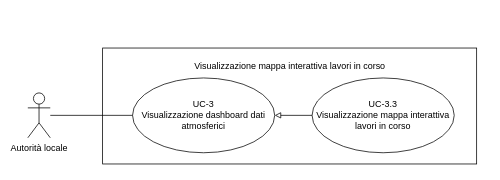
\includegraphics[width=0.65\textwidth]{analisi_dei_requisiti/UC-3.3.png}
	\captionof{figure}{UC-3.3: Visualizzazione \textit{panel} temperatura media nel periodo di tempo selezionato}
\end{center}

\newpage

\subsubsubsection{UC-3.4: Visualizzazione \textit{panel} temperatura in tempo reale}
\begin{itemize}
	\item \textbf{Attore principale}: autorità locale.
	\item \textbf{Precondizioni}:
	      \begin{enumerate}
		      \item l'autorità locale ha effettuato l'accesso al sistema ed esso è in funzione;
		      \item il sistema ha caricato la \href{https://7last.github.io/docs/rtb/documentazione-interna/glossario\#dashboard}{dashboard\textsubscript{G}} relativa ai sensori di temperatura.
	      \end{enumerate}
	\item \textbf{Postcondizioni}: l'autorità locale visualizza un \textit{panel} contenente la temperatura in tempo reale.
	\item \textbf{Scenario principale}:
	      \begin{enumerate}
		      \item l'autorità locale accede alla piattaforma;
		      \item il sistema carica i dati relativi ai sensori interrogando il database;
		      \item l'autorità locale seleziona la visualizzazione della \href{https://7last.github.io/docs/rtb/documentazione-interna/glossario\#dashboard}{dashboard\textsubscript{G}} relativa ai sensori di temperatura.
	      \end{enumerate}
	\item \href{https://7last.github.io/docs/rtb/documentazione-interna/glossario\#user-story}{\textbf{User story}\textsubscript{G}}:
	      come autorità locale desidero poter visualizzare la temperatura in tempo reale in modo da poterne monitorare l'andamento
	      e poterla facilmente confrontare con i dati storici.
\end{itemize}
\begin{center}
	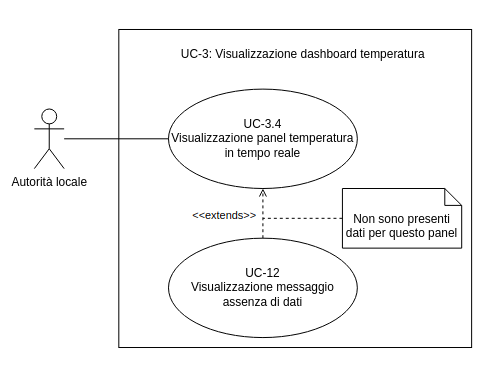
\includegraphics[width=0.65\textwidth]{analisi_dei_requisiti/UC-3.4.png}
	\captionof{figure}{UC-3.4: Visualizzazione \textit{panel} temperatura in tempo reale}
\end{center}

\newpage

\subsubsubsection{UC-3.5: Visualizzazione \textit{panel} temperatura massima nel periodo di tempo selezionato}
\begin{itemize}
	\item \textbf{Attore principale}: autorità locale.
	\item \textbf{Precondizioni}:
	      \begin{enumerate}
		      \item l'autorità locale ha effettuato l'accesso al sistema ed esso è in funzione;
		      \item il sistema ha caricato la \href{https://7last.github.io/docs/rtb/documentazione-interna/glossario\#dashboard}{dashboard\textsubscript{G}} relativa ai sensori di temperatura.
	      \end{enumerate}
	\item \textbf{Postcondizioni}: l'autorità locale visualizza un \textit{panel} contenente la temperatura massima nel periodo di tempo selezionato.
	\item \textbf{Scenario principale}:
	      \begin{enumerate}
		      \item l'autorità locale accede alla piattaforma;
		      \item il sistema carica i dati relativi ai sensori interrogando il database;
		      \item l'autorità locale seleziona la visualizzazione della \href{https://7last.github.io/docs/rtb/documentazione-interna/glossario\#dashboard}{dashboard\textsubscript{G}} relativa ai sensori di temperatura.
	      \end{enumerate}
	\item \href{https://7last.github.io/docs/rtb/documentazione-interna/glossario\#user-story}{\textbf{User story}\textsubscript{G}}:
	      come autorità locale desidero poter visualizzare la temperatura massima nel periodo di tempo selezionato
	      in modo da poterla prendere come riferimento e confrontarla con la temperatura attuale.
\end{itemize}
\begin{center}
	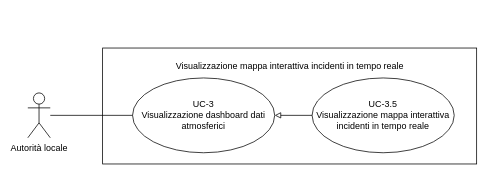
\includegraphics[width=0.65\textwidth]{analisi_dei_requisiti/UC-3.5.png}
	\captionof{figure}{UC-3.5: Visualizzazione \textit{panel} temperatura massima}
\end{center}

\newpage

\subsubsubsection{UC-3.6: Visualizzazione \textit{panel} temperatura minima nel periodo di tempo selezionato}
\begin{itemize}
	\item \textbf{Attore principale}: autorità locale.
	\item \textbf{Precondizioni}:
	      \begin{enumerate}
		      \item l'autorità locale ha effettuato l'accesso al sistema ed esso è in funzione;
		      \item il sistema ha caricato la \href{https://7last.github.io/docs/rtb/documentazione-interna/glossario\#dashboard}{dashboard\textsubscript{G}} relativa ai sensori di temperatura.
	      \end{enumerate}
	\item \textbf{Postcondizioni}: l'autorità locale visualizza un \textit{panel} contenente la temperatura minima nel periodo di tempo selezionato.
	\item \textbf{Scenario principale}:
	      \begin{enumerate}
		      \item l'autorità locale accede alla piattaforma;
		      \item il sistema carica i dati relativi ai sensori interrogando il database;
		      \item l'autorità locale seleziona la visualizzazione della \href{https://7last.github.io/docs/rtb/documentazione-interna/glossario\#dashboard}{dashboard\textsubscript{G}} relativa ai sensori di temperatura.
	      \end{enumerate}
	\item \href{https://7last.github.io/docs/rtb/documentazione-interna/glossario\#user-story}{\textbf{User story}\textsubscript{G}}:
	      come autorità locale desidero poter visualizzare la temperatura minima nel periodo di tempo selezionato
	      in modo da poterla prendere come riferimento e confrontarla con la temperatura attuale.
\end{itemize}
\begin{center}
	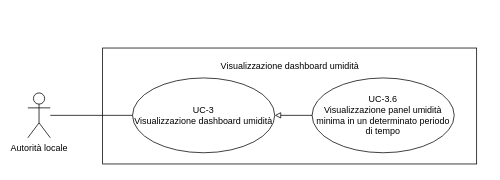
\includegraphics[width=0.65\textwidth]{analisi_dei_requisiti/UC-3.6.png}
	\captionof{figure}{UC-3.6: Visualizzazione \textit{panel} temperatura minima}
\end{center}

\subsubsection{UC-4: Visualizzazione dashboard umidità}
\begin{itemize}
	\item \textbf{Attore principale}: autorità locale.
	\item \textbf{Precondizioni}: l'autorità locale ha effettuato l'accesso al sistema ed esso è in funzione.
	\item \textbf{Postcondizioni}: l'autorità locale visualizza la \href{https://7last.github.io/docs/rtb/documentazione-interna/glossario\#dashboard}{dashboard\textsubscript{G}} relativa
	      ai sensori di umidità presenti nella città.
	\item \textbf{Scenario principale}:
	      \begin{enumerate}
		      \item l'autorità locale accede alla piattaforma;
		      \item il sistema carica i dati trasmessi dai sensori interrogando il database;
		      \item l'autorità locale seleziona la visualizzazione della \href{https://7last.github.io/docs/rtb/documentazione-interna/glossario\#dashboard}{dashboard\textsubscript{G}} relativa ai sensori di umidità.
	      \end{enumerate}
	\item \href{https://7last.github.io/docs/rtb/documentazione-interna/glossario\#user-story}{\textbf{User story}\textsubscript{G}}:
	      come autorità locale desidero poter visualizzare una \href{https://7last.github.io/docs/rtb/documentazione-interna/glossario\#dashboard}{dashboard\textsubscript{G}} relativa ai sensori di umidità presenti nella città, la quale
	      dovrà contenere informazioni utili per monitorare l'andamento dell'umidità sulla base di dati storici e in tempo reale, mostrando
	      anche statistiche come l'umidità media, massima e minima nel periodo di tempo selezionato.
\end{itemize}
\begin{center}
	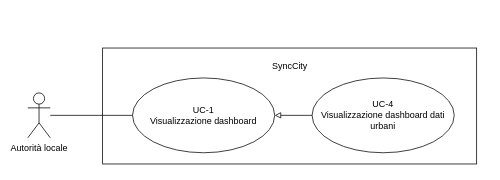
\includegraphics[width=0.75\textwidth]{analisi_dei_requisiti/UC-4.png}
	\captionof{figure}{UC-4: Visualizzazione \href{https://7last.github.io/docs/rtb/documentazione-interna/glossario\#dashboard}{dashboard\textsubscript{G}} umidità}
\end{center}

\newpage

\subsubsubsection{UC-4.1: Visualizzazione grafico time series umidità}
\begin{itemize}
	\item \textbf{Attore principale}: autorità locale.
	\item \textbf{Precondizioni}:
	      \begin{enumerate}
		      \item l'autorità locale ha effettuato l'accesso al sistema ed esso è in funzione;
		      \item il sistema ha caricato la \href{https://7last.github.io/docs/rtb/documentazione-interna/glossario\#dashboard}{dashboard\textsubscript{G}} relativa ai sensori di umidità.
	      \end{enumerate}
	\item \textbf{Postcondizioni}: l'autorità locale visualizza un grafico \href{https://7last.github.io/docs/rtb/documentazione-interna/glossario\#time-series}{time series\textsubscript{G}} contenente le misurazioni storiche di umidità aggregate per 5 minuti.
	\item \textbf{Scenario principale}:
	      \begin{enumerate}
		      \item l'autorità locale accede alla piattaforma;
		      \item il sistema carica i dati relativi ai sensori interrogando il database;
		      \item l'autorità locale seleziona la visualizzazione della \href{https://7last.github.io/docs/rtb/documentazione-interna/glossario\#dashboard}{dashboard\textsubscript{G}} relativa ai sensori di umidità.
	      \end{enumerate}
	\item \href{https://7last.github.io/docs/rtb/documentazione-interna/glossario\#user-story}{\textbf{User story}\textsubscript{G}}:
	      come autorità locale desidero poter visualizzare un grafico \href{https://7last.github.io/docs/rtb/documentazione-interna/glossario\#time-series}{time series\textsubscript{G}} contenente le misurazioni storiche
	      di umidità per poter monitorarne l'andamento nel tempo e facilmente individuare eventuali anomalie.
\end{itemize}
\begin{center}
	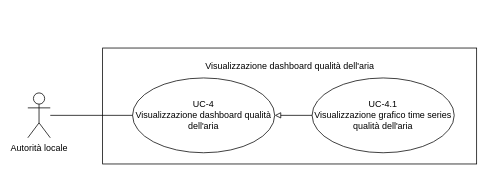
\includegraphics[width=0.65\textwidth]{analisi_dei_requisiti/UC-4.1.png}
	\captionof{figure}{UC-4.1: Visualizzazione grafico \href{https://7last.github.io/docs/rtb/documentazione-interna/glossario\#time-series}{time series\textsubscript{G}} umidità}
\end{center}

\newpage

\subsubsubsection{UC-4.2: Visualizzazione mappa sensori umidità}
\begin{itemize}
	\item \textbf{Attore principale}: autorità locale.
	\item \textbf{Precondizioni}:
	      \begin{enumerate}
		      \item l'autorità locale ha effettuato l'accesso al sistema ed esso è in funzione;
		      \item il sistema ha caricato la \href{https://7last.github.io/docs/rtb/documentazione-interna/glossario\#dashboard}{dashboard\textsubscript{G}} relativa ai sensori di umidità.
	      \end{enumerate}
	\item \textbf{Postcondizioni}: l'autorità locale visualizza una mappa interattiva popolata con dei marker rappresentanti la posizione dei sensori di umidità.
	\item \textbf{Scenario principale}:
	      \begin{enumerate}
		      \item l'autorità locale accede alla piattaforma;
		      \item il sistema carica i dati relativi ai sensori interrogando il database;
		      \item l'autorità locale seleziona la visualizzazione della \href{https://7last.github.io/docs/rtb/documentazione-interna/glossario\#dashboard}{dashboard\textsubscript{G}} relativa ai sensori di umidità.
	      \end{enumerate}
	\item \href{https://7last.github.io/docs/rtb/documentazione-interna/glossario\#user-story}{\textbf{User story}\textsubscript{G}}:
	      come autorità locale desidero poter visualizzare una mappa interattiva popolata con dei marker rappresentanti la posizione dei sensori di umidità
	      e contenenti il loro identificativo. Essa mi consentirà di visualizzare la distribuzione dei sensori di umidità nel territorio ed eventualmente intervenire nel caso in cui siano presenti zone non coperte.
\end{itemize}
\begin{center}
	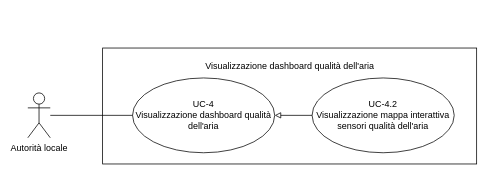
\includegraphics[width=0.6\textwidth]{analisi_dei_requisiti/UC-4.2.png}
	\captionof{figure}{UC-4.2: Visualizzazione mappa interattiva sensori umidità}
\end{center}

\newpage

\subsubsubsection{UC-4.3: Visualizzazione \textit{panel} umidità media nel periodo di tempo selezionato}
\begin{itemize}
	\item \textbf{Attore principale}: autorità locale.
	\item \textbf{Precondizioni}:
	      \begin{enumerate}
		      \item l'autorità locale ha effettuato l'accesso al sistema ed esso è in funzione;
		      \item il sistema ha caricato la \href{https://7last.github.io/docs/rtb/documentazione-interna/glossario\#dashboard}{dashboard\textsubscript{G}} relativa ai sensori di umidità.
	      \end{enumerate}
	\item \textbf{Postcondizioni}: l'autorità locale visualizza un \textit{panel} contenente l'umidità media nel periodo di tempo selezionato.
	\item \textbf{Scenario principale}:
	      \begin{enumerate}
		      \item l'autorità locale accede alla piattaforma;
		      \item il sistema carica i dati relativi ai sensori interrogando il database;
		      \item l'autorità locale seleziona la visualizzazione della \href{https://7last.github.io/docs/rtb/documentazione-interna/glossario\#dashboard}{dashboard\textsubscript{G}} relativa ai sensori di umidità.
	      \end{enumerate}
	\item \href{https://7last.github.io/docs/rtb/documentazione-interna/glossario\#user-story}{\textbf{User story}\textsubscript{G}}: come autorità locale desidero poter visualizzare l'umidità media nel periodo di tempo selezionato
	      in modo da poterne monitorare l'andamento.
\end{itemize}
\begin{center}
	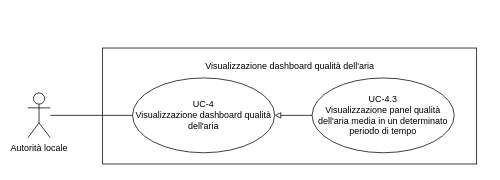
\includegraphics[width=0.65\textwidth]{analisi_dei_requisiti/UC-4.3.png}
	\captionof{figure}{UC-4.3: Visualizzazione \textit{panel} umidità media nel periodo di tempo selezionato}
\end{center}

\newpage

\subsubsubsection{UC-4.4: Visualizzazione \textit{panel} umidità in tempo reale}
\begin{itemize}
	\item \textbf{Attore principale}: autorità locale.
	\item \textbf{Precondizioni}:
	      \begin{enumerate}
		      \item l'autorità locale ha effettuato l'accesso al sistema ed esso è in funzione;
		      \item il sistema ha caricato la \href{https://7last.github.io/docs/rtb/documentazione-interna/glossario\#dashboard}{dashboard\textsubscript{G}} relativa ai sensori di umidità.
	      \end{enumerate}
	\item \textbf{Postcondizioni}: l'autorità locale visualizza un \textit{panel} contenente l'umidità in tempo reale.
	\item \textbf{Scenario principale}:
	      \begin{enumerate}
		      \item l'autorità locale accede alla piattaforma;
		      \item il sistema carica i dati relativi ai sensori interrogando il database;
		      \item l'autorità locale seleziona la visualizzazione della \href{https://7last.github.io/docs/rtb/documentazione-interna/glossario\#dashboard}{dashboard\textsubscript{G}} relativa ai sensori di umidità.
	      \end{enumerate}
	\item \href{https://7last.github.io/docs/rtb/documentazione-interna/glossario\#user-story}{\textbf{User story}\textsubscript{G}}:
	      come autorità locale desidero poter visualizzare l'umidità in tempo reale in modo da poterne monitorare l'andamento
	      e poterla facilmente confrontare con i dati storici.
\end{itemize}
\begin{center}
	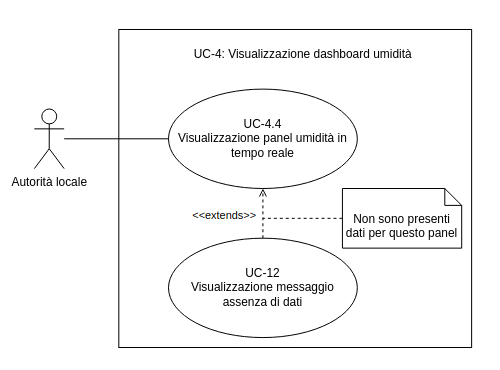
\includegraphics[width=0.65\textwidth]{analisi_dei_requisiti/UC-4.4.png}
	\captionof{figure}{UC-4.4: Visualizzazione \textit{panel} umidità in tempo reale}
\end{center}

\newpage

\subsubsubsection{UC-4.5: Visualizzazione \textit{panel} umidità massima nel periodo di tempo selezionato}
\begin{itemize}
	\item \textbf{Attore principale}: autorità locale.
	\item \textbf{Precondizioni}:
	      \begin{enumerate}
		      \item l'autorità locale ha effettuato l'accesso al sistema ed esso è in funzione;
		      \item il sistema ha caricato la \href{https://7last.github.io/docs/rtb/documentazione-interna/glossario\#dashboard}{dashboard\textsubscript{G}} relativa ai sensori di umidità.
	      \end{enumerate}
	\item \textbf{Postcondizioni}: l'autorità locale visualizza un \textit{panel} contenente l'umidità massima nel periodo di tempo selezionato.
	\item \textbf{Scenario principale}:
	      \begin{enumerate}
		      \item l'autorità locale accede alla piattaforma;
		      \item il sistema carica i dati relativi ai sensori interrogando il database;
		      \item l'autorità locale seleziona la visualizzazione della \href{https://7last.github.io/docs/rtb/documentazione-interna/glossario\#dashboard}{dashboard\textsubscript{G}} relativa ai sensori di umidità.
	      \end{enumerate}
	\item \href{https://7last.github.io/docs/rtb/documentazione-interna/glossario\#user-story}{\textbf{User story}\textsubscript{G}}:
	      come autorità locale desidero poter visualizzare l'umidità massima nel periodo di tempo selezionato
	      in modo da poterla prendere come riferimento e confrontarla con l'umidità attuale.
\end{itemize}
\begin{center}
	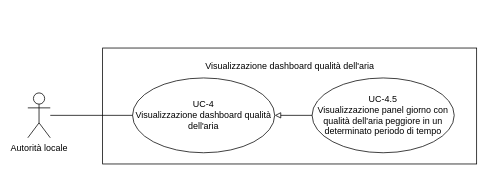
\includegraphics[width=0.6\textwidth]{analisi_dei_requisiti/UC-4.5.png}
	\captionof{figure}{UC-4.5: Visualizzazione \textit{panel} umidità massima}
\end{center}

\newpage

\subsubsubsection{UC-4.6: Visualizzazione \textit{panel} umidità minima nel periodo di tempo selezionato}
\begin{itemize}
	\item \textbf{Attore principale}: autorità locale.
	\item \textbf{Precondizioni}:
	      \begin{enumerate}
		      \item l'autorità locale ha effettuato l'accesso al sistema ed esso è in funzione;
		      \item il sistema ha caricato la \href{https://7last.github.io/docs/rtb/documentazione-interna/glossario\#dashboard}{dashboard\textsubscript{G}} relativa ai sensori di umidità.
	      \end{enumerate}
	\item \textbf{Postcondizioni}: l'autorità locale visualizza un \textit{panel} contenente l'umidità minima nel periodo di tempo selezionato.
	\item \textbf{Scenario principale}:
	      \begin{enumerate}
		      \item l'autorità locale accede alla piattaforma;
		      \item il sistema carica i dati relativi ai sensori interrogando il database;
		      \item l'autorità locale seleziona la visualizzazione della \href{https://7last.github.io/docs/rtb/documentazione-interna/glossario\#dashboard}{dashboard\textsubscript{G}} relativa ai sensori di umidità.
	      \end{enumerate}
	\item \href{https://7last.github.io/docs/rtb/documentazione-interna/glossario\#user-story}{\textbf{User story}\textsubscript{G}}:
	      come autorità locale desidero poter visualizzare l'umidità minima nel periodo di tempo selezionato
	      in modo da poterla prendere come riferimento e confrontarla con l'umidità attuale.
\end{itemize}
\begin{center}
	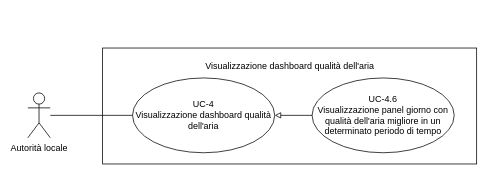
\includegraphics[width=0.6\textwidth]{analisi_dei_requisiti/UC-4.6.png}
	\captionof{figure}{UC-4.6: Visualizzazione \textit{panel} umidità minima}
\end{center}

\subsubsection{UC-5: Visualizzazione dashboard qualità dell'aria}
\begin{itemize}
	\item \textbf{Attore principale}: autorità locale.
	\item \textbf{Precondizioni}: l'autorità locale ha effettuato l'accesso al sistema ed esso è in funzione.
	\item \textbf{Postcondizioni}: l'autorità locale visualizza la \href{https://7last.github.io/docs/rtb/documentazione-interna/glossario\#dashboard}{dashboard\textsubscript{G}} relativa
	      ai sensori di qualità dell'aria presenti nella città.
	\item \textbf{Scenario principale}:
	      \begin{enumerate}
		      \item l'autorità locale accede alla piattaforma;
		      \item il sistema carica i dati trasmessi dai sensori interrogando il database;
		      \item l'autorità locale seleziona la visualizzazione della \href{https://7last.github.io/docs/rtb/documentazione-interna/glossario\#dashboard}{dashboard\textsubscript{G}} relativa ai sensori di qualità dell'aria.
	      \end{enumerate}
	\item \href{https://7last.github.io/docs/rtb/documentazione-interna/glossario\#user-story}{\textbf{User story}\textsubscript{G}}:
	      come autorità locale desidero poter visualizzare una \href{https://7last.github.io/docs/rtb/documentazione-interna/glossario\#dashboard}{dashboard\textsubscript{G}} relativa ai sensori di qualità dell'aria presenti nella città, la quale
	      dovrà contenere informazioni utili per monitorare l'andamento della qualità dell'aria sulla base di dati storici e in tempo reale, mostrando
	      anche statistiche quali il giorno con la qualità dell'aria peggiore e il giorno con la qualità dell'aria migliore nel periodo di tempo selezionato.
\end{itemize}
\begin{center}
	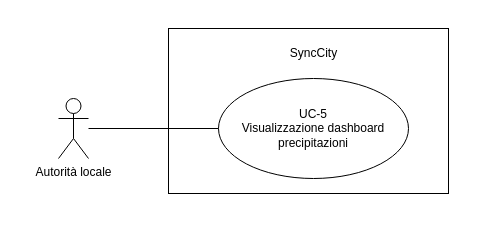
\includegraphics[width=0.75\textwidth]{analisi_dei_requisiti/UC-5.png}
	\captionof{figure}{UC-5: Visualizzazione \href{https://7last.github.io/docs/rtb/documentazione-interna/glossario\#dashboard}{dashboard\textsubscript{G}} qualità dell'aria}
\end{center}

\newpage

\subsubsubsection{UC-5.1: Visualizzazione grafico time series qualità dell'aria}
\begin{itemize}
	\item \textbf{Attore principale}: autorità locale.
	\item \textbf{Precondizioni}:
	      \begin{enumerate}
		      \item l'autorità locale ha effettuato l'accesso al sistema ed esso è in funzione;
		      \item il sistema ha caricato la \href{https://7last.github.io/docs/rtb/documentazione-interna/glossario\#dashboard}{dashboard\textsubscript{G}} relativa ai sensori di qualità dell'aria.
	      \end{enumerate}
	\item \textbf{Postcondizioni}: l'autorità locale visualizza un grafico \href{https://7last.github.io/docs/rtb/documentazione-interna/glossario\#time-series}{time series\textsubscript{G}} contenente le misurazioni storiche
	      di qualità dell'aria aggregate per 5 minuti.
	\item \textbf{Scenario principale}:
	      \begin{enumerate}
		      \item l'autorità locale accede alla piattaforma;
		      \item il sistema carica i dati relativi ai sensori interrogando il database;
		      \item l'autorità locale seleziona la visualizzazione della \href{https://7last.github.io/docs/rtb/documentazione-interna/glossario\#dashboard}{dashboard\textsubscript{G}} relativa ai sensori di qualità dell'aria.
	      \end{enumerate}
	\item \href{https://7last.github.io/docs/rtb/documentazione-interna/glossario\#user-story}{\textbf{User story}\textsubscript{G}}:
	      come autorità locale desidero poter visualizzare un grafico \href{https://7last.github.io/docs/rtb/documentazione-interna/glossario\#time-series}{time series\textsubscript{G}} contenente le misurazioni storiche
	      di qualità dell'aria per poter monitorarne l'andamento nel tempo e facilmente individuare eventuali anomalie.
\end{itemize}
\begin{center}
	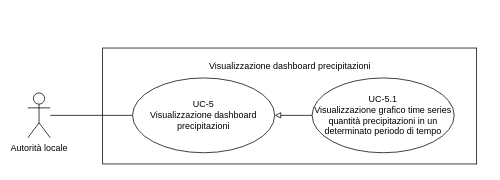
\includegraphics[width=0.6\textwidth]{analisi_dei_requisiti/UC-5.1.png}
	\captionof{figure}{UC-5.1: Visualizzazione grafico \href{https://7last.github.io/docs/rtb/documentazione-interna/glossario\#time-series}{time series\textsubscript{G}} qualità dell'aria}
\end{center}

\newpage

\subsubsubsection{UC-5.2: Visualizzazione mappa interattiva sensori qualità dell'aria}
\begin{itemize}
	\item \textbf{Attore principale}: autorità locale.
	\item \textbf{Precondizioni}:
	      \begin{enumerate}
		      \item l'autorità locale ha effettuato l'accesso al sistema ed esso è in funzione;
		      \item il sistema ha caricato la \href{https://7last.github.io/docs/rtb/documentazione-interna/glossario\#dashboard}{dashboard\textsubscript{G}} relativa ai sensori di qualità dell'aria.
	      \end{enumerate}
	\item \textbf{Postcondizioni}: l'autorità locale visualizza una mappa interattiva popolata con dei marker rappresentanti la posizione dei sensori della qualità dell'aria.
	\item \textbf{Scenario principale}:
	      \begin{enumerate}
		      \item l'autorità locale accede alla piattaforma;
		      \item il sistema carica i dati relativi ai sensori interrogando il database;
		      \item l'autorità locale seleziona la visualizzazione della \href{https://7last.github.io/docs/rtb/documentazione-interna/glossario\#dashboard}{dashboard\textsubscript{G}} relativa ai sensori della qualità dell'aria.
	      \end{enumerate}
	\item \href{https://7last.github.io/docs/rtb/documentazione-interna/glossario\#user-story}{\textbf{User story}\textsubscript{G}}:
	      come autorità locale desidero poter visualizzare una mappa interattiva popolata con dei marker rappresentanti la posizione dei sensori della qualità dell'aria
	      e contenenti il loro identificativo. Essa mi consentirà di visualizzare la distribuzione dei sensori della qualità dell'aria nel territorio ed eventualmente intervenire nel caso in cui siano presenti zone non coperte.
\end{itemize}
\begin{center}
	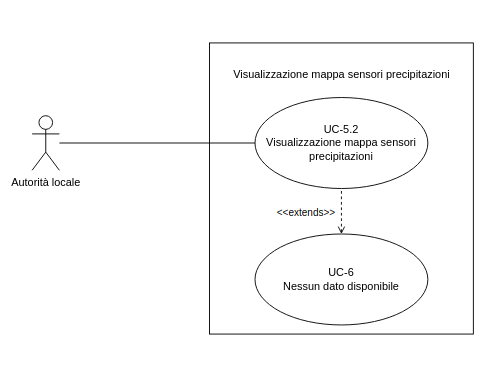
\includegraphics[width=0.6\textwidth]{analisi_dei_requisiti/UC-5.2.png}
	\captionof{figure}{UC-5.2: Visualizzazione mappa interattiva sensori qualità dell'aria}
\end{center}

\newpage

\subsubsubsection{UC-5.3: Visualizzazione \textit{panel} qualità dell'aria media nel periodo di tempo selezionato}
\begin{itemize}
	\item \textbf{Attore principale}: autorità locale.
	\item \textbf{Precondizioni}:
	      \begin{enumerate}
		      \item l'autorità locale ha effettuato l'accesso al sistema ed esso è in funzione;
		      \item il sistema ha caricato la \href{https://7last.github.io/docs/rtb/documentazione-interna/glossario\#dashboard}{dashboard\textsubscript{G}} relativa ai sensori di qualità dell'aria.
	      \end{enumerate}
	\item \textbf{Postcondizioni}: l'autorità locale visualizza un \textit{panel} contenente qualità dell'aria media nel periodo di tempo selezionato.
	\item \textbf{Scenario principale}:
	      \begin{enumerate}
		      \item l'autorità locale accede alla piattaforma;
		      \item il sistema carica i dati relativi ai sensori interrogando il database;
		      \item l'autorità locale seleziona la visualizzazione della \href{https://7last.github.io/docs/rtb/documentazione-interna/glossario\#dashboard}{dashboard\textsubscript{G}} relativa ai sensori di qualità dell'aria.
	      \end{enumerate}
	\item \href{https://7last.github.io/docs/rtb/documentazione-interna/glossario\#user-story}{\textbf{User story}\textsubscript{G}}: come autorità locale desidero poter visualizzare della qualità dell'aria media nel periodo di tempo selezionato
	      in modo da poterne monitorare l'andamento.
\end{itemize}
\begin{center}
	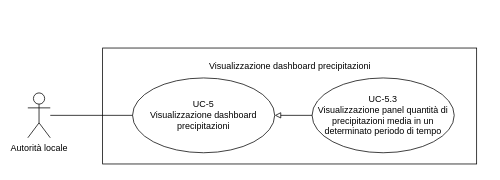
\includegraphics[width=0.6\textwidth]{analisi_dei_requisiti/UC-5.3.png}
	\captionof{figure}{UC-5.3: Visualizzazione \textit{panel} qualità dell'aria media nel periodo di tempo selezionato}
\end{center}

\newpage

\subsubsubsection{UC-5.4: Visualizzazione \textit{panel} qualità dell'aria in tempo reale}
\begin{itemize}
	\item \textbf{Attore principale}: autorità locale.
	\item \textbf{Precondizioni}:
	      \begin{enumerate}
		      \item l'autorità locale ha effettuato l'accesso al sistema ed esso è in funzione;
		      \item il sistema ha caricato la \href{https://7last.github.io/docs/rtb/documentazione-interna/glossario\#dashboard}{dashboard\textsubscript{G}} relativa ai sensori di qualità dell'aria.
	      \end{enumerate}
	\item \textbf{Postcondizioni}: l'autorità locale visualizza un \textit{panel} contenente qualità dell'aria in tempo reale.
	\item \textbf{Scenario principale}:
	      \begin{enumerate}
		      \item l'autorità locale accede alla piattaforma;
		      \item il sistema carica i dati relativi ai sensori interrogando il database;
		      \item l'autorità locale seleziona la visualizzazione della \href{https://7last.github.io/docs/rtb/documentazione-interna/glossario\#dashboard}{dashboard\textsubscript{G}} relativa ai sensori di qualità dell'aria.
	      \end{enumerate}
	\item \href{https://7last.github.io/docs/rtb/documentazione-interna/glossario\#user-story}{\textbf{User story}\textsubscript{G}}:
	      come autorità locale desidero poter visualizzare della qualità dell'aria in tempo reale in modo da poterne monitorare l'andamento
	      e poterla facilmente confrontare con i dati storici.
\end{itemize}
\begin{center}
	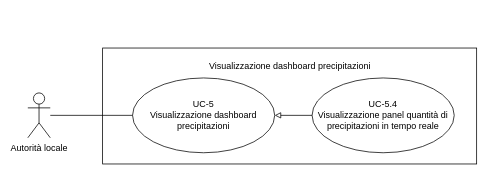
\includegraphics[width=0.6\textwidth]{analisi_dei_requisiti/UC-5.4.png}
	\captionof{figure}{UC-5.4: Visualizzazione \textit{panel} qualità dell'aria in tempo reale}
\end{center}
\subsubsubsection{UC-5.5: Visualizzazione \textit{panel} giorno con qualità dell'aria peggiore nel periodo di tempo selezionato}
\begin{itemize}
	\item \textbf{Attore principale}: autorità locale.
	\item \textbf{Precondizioni}:
	      \begin{enumerate}
		      \item l'autorità locale ha effettuato l'accesso al sistema ed esso è in funzione;
		      \item il sistema ha caricato la \href{https://7last.github.io/docs/rtb/documentazione-interna/glossario\#dashboard}{dashboard\textsubscript{G}} relativa ai sensori di qualità dell'aria.
	      \end{enumerate}
	\item \textbf{Postcondizioni}: l'autorità locale visualizza un \textit{panel} contenente il giorno con la qualità dell'aria peggiore nel periodo di tempo selezionato.
	\item \textbf{Scenario principale}:
	      \begin{enumerate}
		      \item l'autorità locale accede alla piattaforma;
		      \item il sistema carica i dati relativi ai sensori interrogando il database;
		      \item l'autorità locale seleziona la visualizzazione della \href{https://7last.github.io/docs/rtb/documentazione-interna/glossario\#dashboard}{dashboard\textsubscript{G}} relativa ai sensori di qualità dell'aria.
	      \end{enumerate}
	\item \href{https://7last.github.io/docs/rtb/documentazione-interna/glossario\#user-story}{\textbf{User story}\textsubscript{G}}:
	      come autorità locale desidero poter visualizzare il giorno con la qualità dell'aria peggiore nel periodo di tempo selezionato
	      in modo da poterla prendere come riferimento e confrontarla con la qualità dell'aria attuale.
\end{itemize}
\begin{center}
	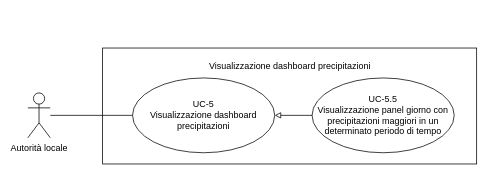
\includegraphics[width=0.6\textwidth]{analisi_dei_requisiti/UC-5.5.png}
	\captionof{figure}{UC-5.5: Visualizzazione \textit{panel} giorno con qualità dell'aria peggiore nel periodo di tempo selezionato}
\end{center}

\newpage

\subsubsubsection{UC-5.6: Visualizzazione \textit{panel} giorno con qualità dell'aria migliore nel periodo di tempo selezionato}
\begin{itemize}
	\item \textbf{Attore principale}: autorità locale.
	\item \textbf{Precondizioni}:
	      \begin{enumerate}
		      \item l'autorità locale ha effettuato l'accesso al sistema ed esso è in funzione;
		      \item il sistema ha caricato la \href{https://7last.github.io/docs/rtb/documentazione-interna/glossario\#dashboard}{dashboard\textsubscript{G}} relativa ai sensori di qualità dell'aria.
	      \end{enumerate}
	\item \textbf{Postcondizioni}: l'autorità locale visualizza un \textit{panel} contenente il giorno con la qualità dell'aria migliore nel periodo di tempo selezionato.
	\item \textbf{Scenario principale}:
	      \begin{enumerate}
		      \item l'autorità locale accede alla piattaforma;
		      \item il sistema carica i dati relativi ai sensori interrogando il database;
		      \item l'autorità locale seleziona la visualizzazione della \href{https://7last.github.io/docs/rtb/documentazione-interna/glossario\#dashboard}{dashboard\textsubscript{G}} relativa ai sensori di qualità dell'aria.
	      \end{enumerate}
	\item \href{https://7last.github.io/docs/rtb/documentazione-interna/glossario\#user-story}{\textbf{User story}\textsubscript{G}}:
	      come autorità locale desidero poter visualizzare il giorno con la qualità dell'aria migliore nel periodo di tempo selezionato
	      in modo da poterla prendere come riferimento e confrontarla con la qualità dell'aria attuale.
\end{itemize}
\begin{center}
	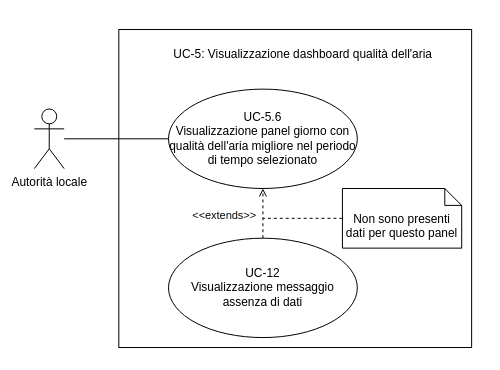
\includegraphics[width=0.6\textwidth]{analisi_dei_requisiti/UC-5.6.png}
	\captionof{figure}{UC-5.6: Visualizzazione \textit{panel} giorno con qualità dell'aria peggiore nel periodo di tempo selezionato}
\end{center}

\subsubsection{UC-6: Visualizzazione dashboard precipitazioni}
\begin{itemize}
	\item \textbf{Attore principale}: autorità locale.
	\item \textbf{Precondizioni}: l'autorità locale ha effettuato l'accesso al sistema ed esso è in funzione.
	\item \textbf{Postcondizioni}: l'autorità locale visualizza la \href{https://7last.github.io/docs/rtb/documentazione-interna/glossario\#dashboard}{dashboard\textsubscript{G}} relativa
	      ai sensori di precipitazioni presenti nella città.
	\item \textbf{Scenario principale}:
	      \begin{enumerate}
		      \item l'autorità locale accede alla piattaforma;
		      \item il sistema carica i dati trasmessi dai sensori interrogando il database;
		      \item l'autorità locale seleziona la visualizzazione della \href{https://7last.github.io/docs/rtb/documentazione-interna/glossario\#dashboard}{dashboard\textsubscript{G}} relativa ai sensori di precipitazioni.
	      \end{enumerate}
	\item \href{https://7last.github.io/docs/rtb/documentazione-interna/glossario\#user-story}{\textbf{User story}\textsubscript{G}}:
	      come autorità locale desidero poter visualizzare una \href{https://7last.github.io/docs/rtb/documentazione-interna/glossario\#dashboard}{dashboard\textsubscript{G}} relativa ai sensori di precipitazioni presenti nella città, la quale
	      dovrà contenere informazioni utili per monitorare l'andamento delle precipitazioni sulla base di dati storici e in tempo reale, mostrando
	      anche statistiche quali quantità di precipitazioni media, massima e minima nel periodo di tempo selezionato.
\end{itemize}
\begin{center}
	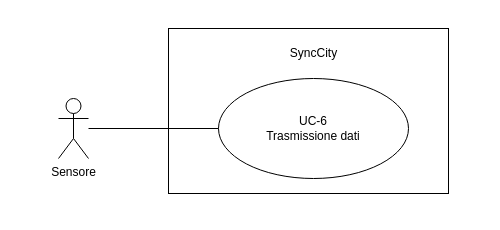
\includegraphics[width=0.75\textwidth]{analisi_dei_requisiti/UC-6.png}
	\captionof{figure}{UC-6: Visualizzazione \href{https://7last.github.io/docs/rtb/documentazione-interna/glossario\#dashboard}{dashboard\textsubscript{G}} precipitazioni}
\end{center}

\newpage

\subsubsubsection{UC-6.1: Visualizzazione grafico time series quantità precipitazioni nel periodo di tempo selezionato}
\begin{itemize}
	\item \textbf{Attore principale}: autorità locale.
	\item \textbf{Precondizioni}:
	      \begin{enumerate}
		      \item l'autorità locale ha effettuato l'accesso al sistema ed esso è in funzione;
		      \item il sistema ha caricato la \href{https://7last.github.io/docs/rtb/documentazione-interna/glossario\#dashboard}{dashboard\textsubscript{G}} relativa ai sensori di precipitazioni
	      \end{enumerate}
	\item \textbf{Postcondizioni}: l'autorità locale visualizza un grafico \href{https://7last.github.io/docs/rtb/documentazione-interna/glossario\#time-series}{time series\textsubscript{G}} contenente le misurazioni storiche
	      di precipitazioni aggregate per 5 minuti.
	\item \textbf{Scenario principale}:
	      \begin{enumerate}
		      \item l'autorità locale accede alla piattaforma;
		      \item il sistema carica i dati relativi ai sensori interrogando il database;
		      \item l'autorità locale seleziona la visualizzazione della \href{https://7last.github.io/docs/rtb/documentazione-interna/glossario\#dashboard}{dashboard\textsubscript{G}} relativa ai sensori di precipitazioni.
	      \end{enumerate}
	\item \href{https://7last.github.io/docs/rtb/documentazione-interna/glossario\#user-story}{\textbf{User story}\textsubscript{G}}:
	      come autorità locale desidero poter visualizzare un grafico \href{https://7last.github.io/docs/rtb/documentazione-interna/glossario\#time-series}{time series\textsubscript{G}} contenente le misurazioni storiche
	      di precipitazioni per poter monitorarne l'andamento nel tempo e facilmente individuare eventuali anomalie.
\end{itemize}
\begin{center}
	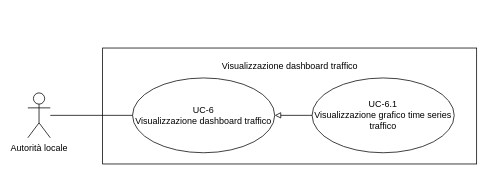
\includegraphics[width=0.6\textwidth]{analisi_dei_requisiti/UC-6.1.png}
	\captionof{figure}{UC-6.1: Visualizzazione grafico \href{https://7last.github.io/docs/rtb/documentazione-interna/glossario\#time-series}{time series\textsubscript{G}} precipitazioni}
\end{center}

\newpage

\subsubsubsection{UC-6.2: Visualizzazione mappa sensori precipitazioni}
\begin{itemize}
	\item \textbf{Attore principale}: autorità locale.
	\item \textbf{Precondizioni}:
	      \begin{enumerate}
		      \item l'autorità locale ha effettuato l'accesso al sistema ed esso è in funzione;
		      \item il sistema ha caricato la \href{https://7last.github.io/docs/rtb/documentazione-interna/glossario\#dashboard}{dashboard\textsubscript{G}} relativa ai sensori di precipitazioni.
	      \end{enumerate}
	\item \textbf{Postcondizioni}: l'autorità locale visualizza una mappa interattiva popolata con dei marker rappresentanti la posizione dei sensori di precipitazioni.
	\item \textbf{Scenario principale}:
	      \begin{enumerate}
		      \item l'autorità locale accede alla piattaforma;
		      \item il sistema carica i dati relativi ai sensori interrogando il database;
		      \item l'autorità locale seleziona la visualizzazione della \href{https://7last.github.io/docs/rtb/documentazione-interna/glossario\#dashboard}{dashboard\textsubscript{G}} relativa ai sensori di precipitazioni.
	      \end{enumerate}
	\item \href{https://7last.github.io/docs/rtb/documentazione-interna/glossario\#user-story}{\textbf{User story}\textsubscript{G}}:
	      come autorità locale desidero poter visualizzare una mappa interattiva popolata con dei marker rappresentanti la posizione dei sensori di precipitazioni
	      e contenenti il loro identificativo. Essa mi consentirà di visualizzare la distribuzione dei sensori di precipitazioni nel territorio ed
	      eventualmente intervenire nel caso in cui siano presenti zone non coperte.
\end{itemize}
\begin{center}
	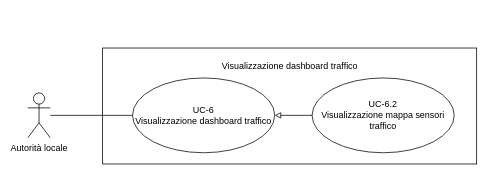
\includegraphics[width=0.6\textwidth]{analisi_dei_requisiti/UC-6.2.png}
	\captionof{figure}{UC-6.2: Visualizzazione mappa interattiva sensori precipitazioni}
\end{center}


\subsubsubsection{UC-6.3: Visualizzazione \textit{panel} quantità di precipitazioni media nel periodo di tempo selezionato}
\begin{itemize}
	\item \textbf{Attore principale}: autorità locale.
	\item \textbf{Precondizioni}:
	      \begin{enumerate}
		      \item l'autorità locale ha effettuato l'accesso al sistema ed esso è in funzione;
		      \item il sistema ha caricato la \href{https://7last.github.io/docs/rtb/documentazione-interna/glossario\#dashboard}{dashboard\textsubscript{G}} relativa ai sensori di precipitazioni.
	      \end{enumerate}
	\item \textbf{Postcondizioni}: l'autorità locale visualizza un \textit{panel} contenente di quantità di precipitazioni media nel periodo di tempo selezionato.
	\item \textbf{Scenario principale}:
	      \begin{enumerate}
		      \item l'autorità locale accede alla piattaforma;
		      \item il sistema carica i dati relativi ai sensori interrogando il database;
		      \item l'autorità locale seleziona la visualizzazione della \href{https://7last.github.io/docs/rtb/documentazione-interna/glossario\#dashboard}{dashboard\textsubscript{G}} relativa ai sensori di precipitazioni.
	      \end{enumerate}
	\item \href{https://7last.github.io/docs/rtb/documentazione-interna/glossario\#user-story}{\textbf{User story}\textsubscript{G}}: come autorità locale desidero poter visualizzare di quantità di precipitazioni media nel periodo di tempo selezionato
	      in modo da poterne monitorare l'andamento.
\end{itemize}
\begin{center}
	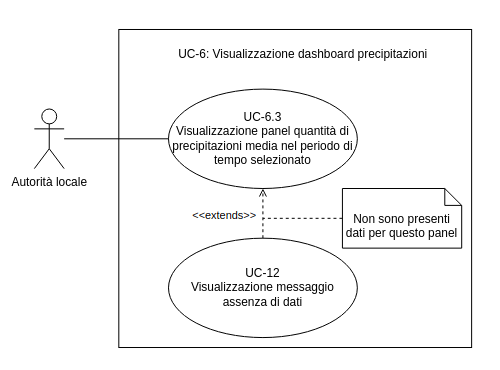
\includegraphics[width=0.6\textwidth]{analisi_dei_requisiti/UC-6.3.png}
	\captionof{figure}{UC-6.3: Visualizzazione \textit{panel} quantità di precipitazioni media nel periodo di tempo selezionato}
\end{center}

\newpage

\subsubsubsection{UC-6.4: Visualizzazione \textit{panel} quantità di precipitazioni in tempo reale}
\begin{itemize}
	\item \textbf{Attore principale}: autorità locale.
	\item \textbf{Precondizioni}:
	      \begin{enumerate}
		      \item l'autorità locale ha effettuato l'accesso al sistema ed esso è in funzione;
		      \item il sistema ha caricato la \href{https://7last.github.io/docs/rtb/documentazione-interna/glossario\#dashboard}{dashboard\textsubscript{G}} relativa ai sensori di precipitazioni.
	      \end{enumerate}
	\item \textbf{Postcondizioni}: l'autorità locale visualizza un \textit{panel} contenente di quantità di precipitazioni in tempo reale.
	\item \textbf{Scenario principale}:
	      \begin{enumerate}
		      \item l'autorità locale accede alla piattaforma;
		      \item il sistema carica i dati relativi ai sensori interrogando il database;
		      \item l'autorità locale seleziona la visualizzazione della \href{https://7last.github.io/docs/rtb/documentazione-interna/glossario\#dashboard}{dashboard\textsubscript{G}} relativa ai sensori di precipitazioni.
	      \end{enumerate}
	\item \href{https://7last.github.io/docs/rtb/documentazione-interna/glossario\#user-story}{\textbf{User story}\textsubscript{G}}:
	      come autorità locale desidero poter visualizzare di quantità di precipitazioni in tempo reale in modo da poterne monitorare l'andamento
	      e poterla facilmente confrontare con i dati storici.
\end{itemize}
\begin{center}
	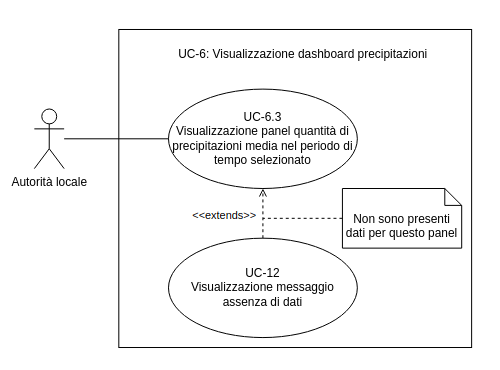
\includegraphics[width=0.6\textwidth]{analisi_dei_requisiti/UC-6.3.png}
	\captionof{figure}{UC-6.3: Visualizzazione \textit{panel} quantità di precipitazioni in tempo reale}
\end{center}

\newpage

\subsubsubsection{UC-6.5: Visualizzazione \textit{panel} giorno con precipitazioni maggiori nel periodo di tempo selezionato}
\begin{itemize}
	\item \textbf{Attore principale}: autorità locale.
	\item \textbf{Precondizioni}:
	      \begin{enumerate}
		      \item l'autorità locale ha effettuato l'accesso al sistema ed esso è in funzione;
		      \item il sistema ha caricato la \href{https://7last.github.io/docs/rtb/documentazione-interna/glossario\#dashboard}{dashboard\textsubscript{G}} relativa ai sensori di precipitazioni.
	      \end{enumerate}
	\item \textbf{Postcondizioni}: l'autorità locale visualizza un \textit{panel} contenente il giorno con la quantità di precipitazioni maggiori nel periodo di tempo selezionato.
	\item \textbf{Scenario principale}:
	      \begin{enumerate}
		      \item l'autorità locale accede alla piattaforma;
		      \item il sistema carica i dati relativi ai sensori interrogando il database;
		      \item l'autorità locale seleziona la visualizzazione della \href{https://7last.github.io/docs/rtb/documentazione-interna/glossario\#dashboard}{dashboard\textsubscript{G}} relativa ai sensori di precipitazioni.
	      \end{enumerate}
	\item \href{https://7last.github.io/docs/rtb/documentazione-interna/glossario\#user-story}{\textbf{User story}\textsubscript{G}}:
	      come autorità locale desidero poter visualizzare il giorno con la quantità di precipitazioni maggiori nel periodo di tempo selezionato
	      e poterla facilmente confrontare con i dati storici.
\end{itemize}
\begin{center}
	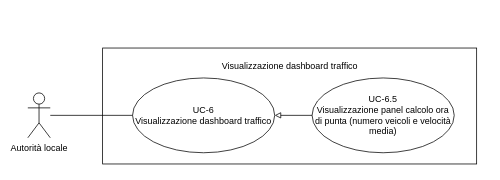
\includegraphics[width=0.6\textwidth]{analisi_dei_requisiti/UC-6.5.png}
	\captionof{figure}{UC-6.5: Visualizzazione \textit{panel} giorno con precipitazioni maggiori nel periodo di tempo selezionato}
\end{center}

\newpage

\subsubsubsection{UC-6.6: Visualizzazione \textit{panel} giorno con precipitazioni minori nel periodo di tempo selezionato}
\begin{itemize}
	\item \textbf{Attore principale}: autorità locale.
	\item \textbf{Precondizioni}:
	      \begin{enumerate}
		      \item l'autorità locale ha effettuato l'accesso al sistema ed esso è in funzione;
		      \item il sistema ha caricato la \href{https://7last.github.io/docs/rtb/documentazione-interna/glossario\#dashboard}{dashboard\textsubscript{G}} relativa ai sensori di precipitazioni.
	      \end{enumerate}
	\item \textbf{Postcondizioni}: l'autorità locale visualizza un \textit{panel} contenente il giorno con la quantità di precipitazioni minori nel periodo di tempo selezionato.
	\item \textbf{Scenario principale}:
	      \begin{enumerate}
		      \item l'autorità locale accede alla piattaforma;
		      \item il sistema carica i dati relativi ai sensori interrogando il database;
		      \item l'autorità locale seleziona la visualizzazione della \href{https://7last.github.io/docs/rtb/documentazione-interna/glossario\#dashboard}{dashboard\textsubscript{G}} relativa ai sensori di precipitazioni.
	      \end{enumerate}
	\item \href{https://7last.github.io/docs/rtb/documentazione-interna/glossario\#user-story}{\textbf{User story}\textsubscript{G}}:
	      come autorità locale desidero poter visualizzare il giorno con la quantità di precipitazioni minori nel periodo di tempo selezionato
	      e poterla facilmente confrontare con i dati storici.
\end{itemize}
\begin{center}
	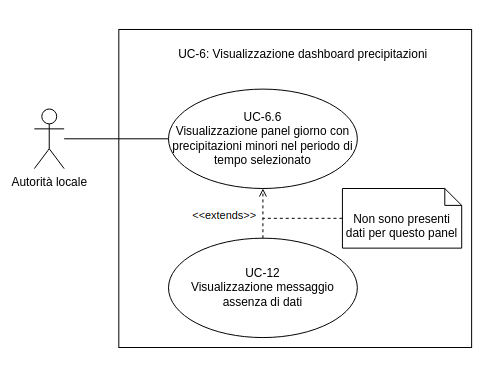
\includegraphics[width=0.6\textwidth]{analisi_dei_requisiti/UC-6.6.png}
	\captionof{figure}{UC-6.6: Visualizzazione \textit{panel} giorno con precipitazioni minori nel periodo di tempo selezionato}
\end{center}

\subsubsection{UC-7: Visualizzazione dashboard traffico}
\begin{itemize}
	\item \textbf{Attore principale}: autorità locale.
	\item \textbf{Precondizioni}: l'autorità locale ha effettuato l'accesso al sistema ed esso è in funzione.
	\item \textbf{Postcondizioni}: l'autorità locale visualizza la \href{https://7last.github.io/docs/rtb/documentazione-interna/glossario\#dashboard}{dashboard\textsubscript{G}} relativa
	      ai sensori di traffico presenti nella città.
	\item \textbf{Scenario principale}:
	      \begin{enumerate}
		      \item l'autorità locale accede alla piattaforma;
		      \item il sistema carica i dati trasmessi dai sensori interrogando il database;
		      \item l'autorità locale seleziona la visualizzazione della \href{https://7last.github.io/docs/rtb/documentazione-interna/glossario\#dashboard}{dashboard\textsubscript{G}} relativa ai sensori di traffico.
	      \end{enumerate}
	\item \href{https://7last.github.io/docs/rtb/documentazione-interna/glossario\#user-story}{\textbf{User story}\textsubscript{G}}:
	      come autorità locale desidero poter visualizzare una \href{https://7last.github.io/docs/rtb/documentazione-interna/glossario\#dashboard}{dashboard\textsubscript{G}} relativa ai sensori di traffico presenti nella città, la quale
	      dovrà contenere informazioni utili per monitorare l'andamento del traffico sulla base di dati storici e in tempo reale, mostrando
	      anche statistiche quali numero di veicoli in tempo reale, velocità media in tempo reale e calcolo dell'ora di punta (basato su numero veicoli e velocità media).
\end{itemize}
\begin{center}
	\includegraphics[width=0.75\textwidth]{analisi_dei_requisiti/UC-7.png}
	\captionof{figure}{UC-7: Visualizzazione \href{https://7last.github.io/docs/rtb/documentazione-interna/glossario\#dashboard}{dashboard\textsubscript{G}} traffico}
\end{center}

\newpage

\subsubsubsection{UC-7.1: Visualizzazione grafico time series traffico}
\begin{itemize}
	\item \textbf{Attore principale}: autorità locale.
	\item \textbf{Precondizioni}:
	      \begin{enumerate}
		      \item l'autorità locale ha effettuato l'accesso al sistema ed esso è in funzione;
		      \item il sistema ha caricato la \href{https://7last.github.io/docs/rtb/documentazione-interna/glossario\#dashboard}{dashboard\textsubscript{G}} relativa ai sensori di traffico.
	      \end{enumerate}
	\item \textbf{Postcondizioni}: l'autorità locale visualizza un grafico \href{https://7last.github.io/docs/rtb/documentazione-interna/glossario\#time-series}{time series\textsubscript{G}} contenente le misurazioni storiche di traffico aggregate per 5 minuti.
	\item \textbf{Scenario principale}:
	      \begin{enumerate}
		      \item l'autorità locale accede alla piattaforma;
		      \item il sistema carica i dati relativi ai sensori interrogando il database;
		      \item l'autorità locale seleziona la visualizzazione della \href{https://7last.github.io/docs/rtb/documentazione-interna/glossario\#dashboard}{dashboard\textsubscript{G}} relativa ai sensori di traffico.
	      \end{enumerate}
	\item \href{https://7last.github.io/docs/rtb/documentazione-interna/glossario\#user-story}{\textbf{User story}\textsubscript{G}}:
	      come autorità locale desidero poter visualizzare un grafico \href{https://7last.github.io/docs/rtb/documentazione-interna/glossario\#time-series}{time series\textsubscript{G}} contenente le misurazioni storiche
	      di traffico per poter monitorarne l'andamento nel tempo e facilmente individuare eventuali anomalie
	      o congestioni.
\end{itemize}
\begin{center}
	\includegraphics[width=0.6\textwidth]{analisi_dei_requisiti/UC-7.1.png}
	\captionof{figure}{UC-7.1: Visualizzazione grafico \href{https://7last.github.io/docs/rtb/documentazione-interna/glossario\#time-series}{time series\textsubscript{G}} traffico}
\end{center}

\newpage

\subsubsubsection{UC-7.2: Visualizzazione mappa sensori traffico}
\begin{itemize}
	\item \textbf{Attore principale}: autorità locale.
	\item \textbf{Precondizioni}:
	      \begin{enumerate}
		      \item l'autorità locale ha effettuato l'accesso al sistema ed esso è in funzione;
		      \item il sistema ha caricato la \href{https://7last.github.io/docs/rtb/documentazione-interna/glossario\#dashboard}{dashboard\textsubscript{G}} relativa ai sensori di traffico.
	      \end{enumerate}
	\item \textbf{Postcondizioni}: l'autorità locale visualizza una mappa interattiva popolata con dei marker rappresentanti la posizione dei sensori del traffico.
	\item \textbf{Scenario principale}:
	      \begin{enumerate}
		      \item l'autorità locale accede alla piattaforma;
		      \item il sistema carica i dati relativi ai sensori interrogando il database;
		      \item l'autorità locale seleziona la visualizzazione della \href{https://7last.github.io/docs/rtb/documentazione-interna/glossario\#dashboard}{dashboard\textsubscript{G}} relativa ai sensori del traffico.
	      \end{enumerate}
	\item \href{https://7last.github.io/docs/rtb/documentazione-interna/glossario\#user-story}{\textbf{User story}\textsubscript{G}}:
	      come autorità locale desidero poter visualizzare una mappa interattiva popolata con dei marker rappresentanti la posizione dei sensori del traffico
	      e contenenti il loro identificativo. Essa mi consentirà di visualizzare la distribuzione dei sensori del traffico nel territorio ed eventualmente intervenire nel caso in cui siano presenti zone non coperte.
\end{itemize}
\begin{center}
	\includegraphics[width=0.6\textwidth]{analisi_dei_requisiti/UC-7.2.png}
	\captionof{figure}{UC-7.2: Visualizzazione mappa interattiva sensori traffico}
\end{center}

\newpage

\subsubsubsection{UC-7.3: Visualizzazione \textit{panel} numero veicoli in tempo reale}
\begin{itemize}
	\item \textbf{Attore principale}: autorità locale.
	\item \textbf{Precondizioni}:
	      \begin{enumerate}
		      \item l'autorità locale ha effettuato l'accesso al sistema ed esso è in funzione;
		      \item il sistema ha caricato la \href{https://7last.github.io/docs/rtb/documentazione-interna/glossario\#dashboard}{dashboard\textsubscript{G}} relativa ai sensori di traffico.
	      \end{enumerate}
	\item \textbf{Postcondizioni}: l'autorità locale visualizza un \textit{panel} contenente il numero di veicoli in tempo reale.
	\item \textbf{Scenario principale}:
	      \begin{enumerate}
		      \item l'autorità locale accede alla piattaforma;
		      \item il sistema carica i dati relativi ai sensori interrogando il database;
		      \item l'autorità locale seleziona la visualizzazione della \href{https://7last.github.io/docs/rtb/documentazione-interna/glossario\#dashboard}{dashboard\textsubscript{G}} relativa ai sensori di traffico.
	      \end{enumerate}
	\item \href{https://7last.github.io/docs/rtb/documentazione-interna/glossario\#user-story}{\textbf{User story}\textsubscript{G}}:
	      come autorità locale desidero poter visualizzare del numero di veicoli in tempo reale in modo da poterne monitorare l'andamento
	      e poterla facilmente confrontare con i dati storici.
\end{itemize}
\begin{center}
	\includegraphics[width=0.6\textwidth]{analisi_dei_requisiti/UC-7.3.png}
	\captionof{figure}{UC-7.3: Visualizzazione \textit{panel} numero di veicoli in tempo reale}
\end{center}

\newpage

\subsubsubsection{UC-7.4: Visualizzazione \textit{panel} velocità media in tempo reale}
\begin{itemize}
	\item \textbf{Attore principale}: autorità locale.
	\item \textbf{Precondizioni}:
	      \begin{enumerate}
		      \item l'autorità locale ha effettuato l'accesso al sistema ed esso è in funzione;
		      \item il sistema ha caricato la \href{https://7last.github.io/docs/rtb/documentazione-interna/glossario\#dashboard}{dashboard\textsubscript{G}} relativa ai sensori di traffico.
	      \end{enumerate}
	\item \textbf{Postcondizioni}: l'autorità locale visualizza un \textit{panel} contenente la velocità media in tempo reale.
	\item \textbf{Scenario principale}:
	      \begin{enumerate}
		      \item l'autorità locale accede alla piattaforma;
		      \item il sistema carica i dati relativi ai sensori interrogando il database;
		      \item l'autorità locale seleziona la visualizzazione della \href{https://7last.github.io/docs/rtb/documentazione-interna/glossario\#dashboard}{dashboard\textsubscript{G}} relativa ai sensori di traffico.
	      \end{enumerate}
	\item \href{https://7last.github.io/docs/rtb/documentazione-interna/glossario\#user-story}{\textbf{User story}\textsubscript{G}}:
	      come autorità locale desidero poter visualizzare della velocità media in tempo reale in modo da poterne monitorare l'andamento
	      e poterla facilmente confrontare con i dati storici.
\end{itemize}
\begin{center}
	\includegraphics[width=0.6\textwidth]{analisi_dei_requisiti/UC-7.4.png}
	\captionof{figure}{UC-7.4: Visualizzazione \textit{panel} velocità media in tempo reale}
\end{center}

\newpage

\subsubsubsection{UC-7.5: Visualizzazione \textit{panel} calcolo ora di punta}
\begin{itemize}
	\item \textbf{Attore principale}: autorità locale.
	\item \textbf{Precondizioni}:
	      \begin{enumerate}
		      \item l'autorità locale ha effettuato l'accesso al sistema ed esso è in funzione;
		      \item il sistema ha caricato la \href{https://7last.github.io/docs/rtb/documentazione-interna/glossario\#dashboard}{dashboard\textsubscript{G}} relativa ai sensori di traffico.
	      \end{enumerate}
	\item \textbf{Postcondizioni}: l'autorità locale visualizza un \textit{panel} contenente il calcolo dell'ora di punta basato sul numero di veicoli e sulla velocità media.
	\item \textbf{Scenario principale}:
	      \begin{enumerate}
		      \item l'autorità locale accede alla piattaforma;
		      \item il sistema carica i dati relativi ai sensori interrogando il database;
		      \item l'autorità locale seleziona la visualizzazione della \href{https://7last.github.io/docs/rtb/documentazione-interna/glossario\#dashboard}{dashboard\textsubscript{G}} relativa ai sensori di traffico.
	      \end{enumerate}
	\item \href{https://7last.github.io/docs/rtb/documentazione-interna/glossario\#user-story}{\textbf{User story}\textsubscript{G}}:
	      come autorità locale desidero poter visualizzare il calcolo dell'ora di punta basato sul numero di veicoli e sulla velocità media in modo da poter monitorare
	      l'andamento del traffico e poterlo confrontare con i dati storici.
\end{itemize}
\begin{center}
	\includegraphics[width=0.6\textwidth]{analisi_dei_requisiti/UC-7.5.png}
	\captionof{figure}{UC-7.5: Visualizzazione \textit{panel} calcolo ora di punta}
\end{center}


\subsubsection{UC-8: Visualizzazione dashboard colonnine di ricarica}
\begin{itemize}
	\item \textbf{Attore principale}: autorità locale.
	\item \textbf{Precondizioni}: l'autorità locale ha effettuato l'accesso al sistema ed esso è in funzione.
	\item \textbf{Postcondizioni}: l'autorità locale visualizza la \href{https://7last.github.io/docs/rtb/documentazione-interna/glossario\#dashboard}{dashboard\textsubscript{G}} relativa
	      alle colonnine di ricarica presenti nella città.
	\item \textbf{Scenario principale}:
	      \begin{enumerate}
		      \item l'autorità locale accede alla piattaforma;
		      \item il sistema carica i dati trasmessi dai sensori interrogando il database;
		      \item l'autorità locale seleziona la visualizzazione della \href{https://7last.github.io/docs/rtb/documentazione-interna/glossario\#dashboard}{dashboard\textsubscript{G}} relativa alle colonnine di ricarica.
	      \end{enumerate}
	\item \href{https://7last.github.io/docs/rtb/documentazione-interna/glossario\#user-story}{\textbf{User story}\textsubscript{G}}:
	      come autorità locale desidero poter visualizzare una \href{https://7last.github.io/docs/rtb/documentazione-interna/glossario\#dashboard}{dashboard\textsubscript{G}} relativa alle colonnine di ricarica presenti nella città, la quale
	      dovrà contenere informazioni riguardo il loro stato di funzionamento e manutenzione.
\end{itemize}
\begin{center}
	\includegraphics[width=0.75\textwidth]{analisi_dei_requisiti/UC-8.png}
	\captionof{figure}{UC-8: Visualizzazione \href{https://7last.github.io/docs/rtb/documentazione-interna/glossario\#dashboard}{dashboard\textsubscript{G}} colonnine di ricarica}
\end{center}

\newpage

\subsubsubsection{UC-8.1: Visualizzazione mappa colonnine di ricarica con stato}
\begin{itemize}
	\item \textbf{Attore principale}: autorità locale.
	\item \textbf{Precondizioni}:
	      \begin{enumerate}
		      \item l'autorità locale ha effettuato l'accesso al sistema ed esso è in funzione;
		      \item il sistema ha caricato la \href{https://7last.github.io/docs/rtb/documentazione-interna/glossario\#dashboard}{dashboard\textsubscript{G}} relativa alle colonnine di ricarica.
	      \end{enumerate}
	\item \textbf{Postcondizioni}: l'autorità locale visualizza una mappa interattiva popolata con dei marker rappresentanti la posizione delle colonnine di ricarica.
	\item \textbf{Scenario principale}:
	      \begin{enumerate}
		      \item l'autorità locale accede alla piattaforma;
		      \item il sistema carica i dati relativi ai sensori interrogando il database;
		      \item l'autorità locale seleziona la visualizzazione della \href{https://7last.github.io/docs/rtb/documentazione-interna/glossario\#dashboard}{dashboard\textsubscript{G}} relativa delle colonnine di ricarica.
	      \end{enumerate}
	\item \href{https://7last.github.io/docs/rtb/documentazione-interna/glossario\#user-story}{\textbf{User story}\textsubscript{G}}:
	      come autorità locale desidero poter visualizzare una mappa interattiva popolata con dei marker rappresentanti la posizione delle colonnine di ricarica
	      contenenti il loro identificativo e lo stato di funzionamento. Essa mi consentirà di visualizzare la distribuzione delle colonnine di ricarica nel territorio
	      ed eventualmente intervenire nel caso in cui vi siano dei guasti.
\end{itemize}
\begin{center}
	\includegraphics[width=0.6\textwidth]{analisi_dei_requisiti/UC-8.1.png}
	\captionof{figure}{UC-8.1: Visualizzazione mappa interattiva sensori colonnine di ricarica}
\end{center}

\newpage

\subsubsubsection{UC-8.2: Visualizzazione \textit{panel} numero colonnine di ricarica per stato in tempo reale}
\begin{itemize}
	\item \textbf{Attore principale}: autorità locale.
	\item \textbf{Precondizioni}:
	      \begin{enumerate}
		      \item l'autorità locale ha effettuato l'accesso al sistema ed esso è in funzione;
		      \item il sistema ha caricato la \href{https://7last.github.io/docs/rtb/documentazione-interna/glossario\#dashboard}{dashboard\textsubscript{G}} relativa ai dati atmosferici.
	      \end{enumerate}
	\item \textbf{Postcondizioni}: l'autorità locale visualizza un \textit{panel} contenente il conteggio delle colonnine di ricarica suddivise per stato di funzionamento.
	\item \textbf{Scenario principale}:
	      \begin{enumerate}
		      \item l'autorità locale accede alla piattaforma;
		      \item il sistema carica i dati relativi ai sensori interrogando il database;
		      \item l'autorità locale seleziona la visualizzazione della \href{https://7last.github.io/docs/rtb/documentazione-interna/glossario\#dashboard}{dashboard\textsubscript{G}} relativa alle colonnine di ricarica.
	      \end{enumerate}
	\item \href{https://7last.github.io/docs/rtb/documentazione-interna/glossario\#user-story}{\textbf{User story}\textsubscript{G}}:
	      come autorità locale desidero poter visualizzare un \textit{panel} contenente il conteggio delle colonnine di ricarica suddivise per stato di funzionamento
	      per poterle monitorare e intervenire in caso di guasti.
\end{itemize}
\begin{center}
	\includegraphics[width=0.6\textwidth]{analisi_dei_requisiti/UC-8.2.png}
	\captionof{figure}{UC-8.2: Visualizzazione \textit{panel} numero colonnine di ricarica per stato}
\end{center}

\subsubsection{UC-9: Visualizzazione dashboard parcheggi}
\begin{itemize}
	\item \textbf{Attore principale}: autorità locale.
	\item \textbf{Precondizioni}: l'autorità locale ha effettuato l'accesso al sistema ed esso è in funzione.
	\item \textbf{Postcondizioni}: l'autorità locale visualizza la \href{https://7last.github.io/docs/rtb/documentazione-interna/glossario\#dashboard}{dashboard\textsubscript{G}} relativa
	      ai parcheggi presenti nella città.
	\item \textbf{Scenario principale}:
	      \begin{enumerate}
		      \item l'autorità locale accede alla piattaforma;
		      \item il sistema carica i dati trasmessi dai sensori interrogando il database;
		      \item l'autorità locale seleziona la visualizzazione della \href{https://7last.github.io/docs/rtb/documentazione-interna/glossario\#dashboard}{dashboard\textsubscript{G}} relativa ai parcheggi.
	      \end{enumerate}
	\item \href{https://7last.github.io/docs/rtb/documentazione-interna/glossario\#user-story}{\textbf{User story}\textsubscript{G}}:
	      come autorità locale desidero poter visualizzare una \href{https://7last.github.io/docs/rtb/documentazione-interna/glossario\#dashboard}{dashboard\textsubscript{G}} relativa ai parcheggi presenti nella città, la quale
	      dovrà contenere informazioni utili per monitorare lo stato di occupazione dei parcheggi sulla base di dati storici e in tempo reale,
	      in modo da poter individuare eventuali zone di criticità e intervenire per aumentare la disponibilità di parcheggi.
\end{itemize}
\begin{center}
	\includegraphics[width=0.75\textwidth]{analisi_dei_requisiti/UC-9.png}
	\captionof{figure}{UC-9: Visualizzazione \href{https://7last.github.io/docs/rtb/documentazione-interna/glossario\#dashboard}{dashboard\textsubscript{G}} parcheggi}
\end{center}

\newpage

\subsubsubsection{UC-9.1: Visualizzazione mappa interattiva parcheggi con rispettivo stato di occupazione}
\begin{itemize}
	\item \textbf{Attore principale}: autorità locale.
	\item \textbf{Precondizioni}:
	      \begin{enumerate}
		      \item l'autorità locale ha effettuato l'accesso al sistema ed esso è in funzione;
		      \item il sistema ha caricato la \href{https://7last.github.io/docs/rtb/documentazione-interna/glossario\#dashboard}{dashboard\textsubscript{G}} relativa ai parcheggi con rispettivo stato di occupazione.
	      \end{enumerate}
	\item \textbf{Postcondizioni}: l'autorità locale visualizza una mappa interattiva popolata con dei marker rappresentanti la posizione dei parcheggi con rispettivo stato di occupazione.
	\item \textbf{Scenario principale}:
	      \begin{enumerate}
		      \item l'autorità locale accede alla piattaforma;
		      \item il sistema carica i dati relativi ai sensori interrogando il database;
		      \item l'autorità locale seleziona la visualizzazione della \href{https://7last.github.io/docs/rtb/documentazione-interna/glossario\#dashboard}{dashboard\textsubscript{G}} relativa ai parcheggi.
	      \end{enumerate}
	\item \href{https://7last.github.io/docs/rtb/documentazione-interna/glossario\#user-story}{\textbf{User story}\textsubscript{G}}:
	      come autorità locale desidero poter visualizzare una mappa interattiva popolata con dei marker rappresentanti la posizione dei parcheggi con rispettivo stato di occupazione
	      e contenenti il loro identificativo. Essa consentirà di individuare facilmente le zone con maggiore affluenza ed eventualmente intervenire per aumentare la disponibilità di parcheggi.
\end{itemize}
\begin{center}
	\includegraphics[width=0.75\textwidth]{analisi_dei_requisiti/UC-9.1.png}
	\captionof{figure}{UC-9.1: Visualizzazione mappa interattiva sensori parcheggi con rispettivo stato di occupazione}
\end{center}

\subsubsubsection{UC-9.2: Visualizzazione \textit{panel} con conteggio parcheggi per stato in tempo reale}
\begin{itemize}
	\item \textbf{Attore principale}: autorità locale.
	\item \textbf{Precondizioni}:
	      \begin{enumerate}
		      \item l'autorità locale ha effettuato l'accesso al sistema ed esso è in funzione;
		      \item il sistema ha caricato la \href{https://7last.github.io/docs/rtb/documentazione-interna/glossario\#dashboard}{dashboard\textsubscript{G}} relativa ai parcheggi.
	      \end{enumerate}
	\item \textbf{Postcondizioni}: l'autorità locale visualizza un \textit{panel} contenente i parcheggi con rispettivo stato di occupazione in tempo reale.
	\item \textbf{Scenario principale}:
	      \begin{enumerate}
		      \item l'autorità locale accede alla piattaforma;
		      \item il sistema carica i dati relativi ai sensori interrogando il database;
		      \item l'autorità locale seleziona la visualizzazione della \href{https://7last.github.io/docs/rtb/documentazione-interna/glossario\#dashboard}{dashboard\textsubscript{G}} relativa ai parcheggi con rispettivo stato di occupazione.
	      \end{enumerate}
	\item \href{https://7last.github.io/docs/rtb/documentazione-interna/glossario\#user-story}{\textbf{User story}\textsubscript{G}}:
	      come autorità locale desidero poter visualizzare i parcheggi con rispettivo stato di occupazione in tempo reale in modo da poterne monitorare l'andamento
	      e poterla facilmente confrontare con i dati storici.
\end{itemize}
\begin{center}
	\includegraphics[width=0.75\textwidth]{analisi_dei_requisiti/UC-9.2.png}
	\captionof{figure}{UC-9.2: Visualizzazione \textit{panel} parcheggi con rispettivo stato di occupazione in tempo reale}
\end{center}
\newpage
\subsubsection{UC-10: Visualizzazione dashboard isole ecologiche}
\begin{itemize}
	\item \textbf{Attore principale}: autorità locale.
	\item \textbf{Precondizioni}: l'autorità locale ha effettuato l'accesso al sistema ed esso è in funzione.
	\item \textbf{Postcondizioni}: l'autorità locale visualizza la \href{https://7last.github.io/docs/rtb/documentazione-interna/glossario\#dashboard}{dashboard\textsubscript{G}} relativa
	      alle isole ecologiche presenti nella città.
	\item \textbf{Scenario principale}:
	      \begin{enumerate}
		      \item l'autorità locale accede alla piattaforma;
		      \item il sistema carica i dati trasmessi dai sensori interrogando il database;
		      \item l'autorità locale seleziona la visualizzazione della \href{https://7last.github.io/docs/rtb/documentazione-interna/glossario\#dashboard}{dashboard\textsubscript{G}} relativa alle isole ecologiche.
	      \end{enumerate}
	\item \href{https://7last.github.io/docs/rtb/documentazione-interna/glossario\#user-story}{\textbf{User story}\textsubscript{G}}:
	      come autorità locale desidero poter visualizzare una \href{https://7last.github.io/docs/rtb/documentazione-interna/glossario\#dashboard}{dashboard\textsubscript{G}} relativa alle isole ecologiche presenti nella città, la quale
	      dovrà contenere informazioni utili per monitorare il loro stato di riempimento. In questo modo potrò intervenire
	      per poter svuotare le isole ecologiche piene.
\end{itemize}
\begin{center}
	\includegraphics[width=0.75\textwidth]{analisi_dei_requisiti/UC-10.png}
	\captionof{figure}{UC-10: Visualizzazione \href{https://7last.github.io/docs/rtb/documentazione-interna/glossario\#dashboard}{dashboard\textsubscript{G}} isole ecologiche}
\end{center}

\newpage

\subsubsubsection{UC-10.1: Visualizzazione \textit{panel} con riempimento isole ecologiche in tempo reale}
\begin{itemize}
	\item \textbf{Attore principale}: autorità locale.
	\item \textbf{Precondizioni}:
	      \begin{enumerate}
		      \item l'autorità locale ha effettuato l'accesso al sistema ed esso è in funzione;
		      \item il sistema ha caricato la \href{https://7last.github.io/docs/rtb/documentazione-interna/glossario\#dashboard}{dashboard\textsubscript{G}} relativa alle isole ecologiche.
	      \end{enumerate}
	\item \textbf{Postcondizioni}: l'autorità locale visualizza un \textit{panel} contenente il riempimento in percentuale delle isole ecologiche in tempo reale.
	\item \textbf{Scenario principale}:
	      \begin{enumerate}
		      \item l'autorità locale accede alla piattaforma;
		      \item il sistema carica i dati relativi ai sensori interrogando il database;
		      \item l'autorità locale seleziona la visualizzazione della \href{https://7last.github.io/docs/rtb/documentazione-interna/glossario\#dashboard}{dashboard\textsubscript{G}} relativa alle isole ecologiche.
	      \end{enumerate}
	\item \href{https://7last.github.io/docs/rtb/documentazione-interna/glossario\#user-story}{\textbf{User story}\textsubscript{G}}:
	      come autorità locale desidero poter visualizzare il riempimento in percentuale delle isole ecologiche in tempo reale in modo da poterne monitorare l'andamento
	      ed eventualmente intervenire per svuotarle.
\end{itemize}
\begin{center}
	\includegraphics[width=0.6\textwidth]{analisi_dei_requisiti/UC-10.1.png}
	\captionof{figure}{UC-10.1: Visualizzazione \textit{panel} riempimento isole ecologiche in tempo reale}
\end{center}

\newpage

\subsubsubsection{UC-10.2: Visualizzazione mappa interattiva isole ecologiche}
\begin{itemize}
	\item \textbf{Attore principale}: autorità locale.
	\item \textbf{Precondizioni}:
	      \begin{enumerate}
		      \item l'autorità locale ha effettuato l'accesso al sistema ed esso è in funzione;
		      \item il sistema ha caricato la \href{https://7last.github.io/docs/rtb/documentazione-interna/glossario\#dashboard}{dashboard\textsubscript{G}} relativa ai sensori di isole ecologiche.
	      \end{enumerate}
	\item \textbf{Postcondizioni}: l'autorità locale visualizza una mappa interattiva popolata con dei marker rappresentanti la posizione dei sensori delle isole ecologiche.
	\item \textbf{Scenario principale}:
	      \begin{enumerate}
		      \item l'autorità locale accede alla piattaforma;
		      \item il sistema carica i dati relativi ai sensori interrogando il database;
		      \item l'autorità locale seleziona la visualizzazione della \href{https://7last.github.io/docs/rtb/documentazione-interna/glossario\#dashboard}{dashboard\textsubscript{G}} relativa ai sensori delle isole ecologiche piene.
	      \end{enumerate}
	\item \href{https://7last.github.io/docs/rtb/documentazione-interna/glossario\#user-story}{\textbf{User story}\textsubscript{G}}:
	      come autorità locale desidero poter visualizzare una mappa interattiva popolata con dei marker rappresentanti la posizione dei sensori delle isole ecologiche
	      contenenti il loro identificativo. Essa mi consentirà di visualizzare la distribuzione delle isole ecologiche nel territorio.
\end{itemize}
\begin{center}
	\includegraphics[width=0.6\textwidth]{analisi_dei_requisiti/UC-10.2.png}
	\captionof{figure}{UC-10.2: Visualizzazione mappa interattiva sensori isole ecologiche}
\end{center}

\newpage

\subsubsubsection{UC-10.3: Visualizzazione grafico time series isole ecologiche}
\begin{itemize}
	\item \textbf{Attore principale}: autorità locale.
	\item \textbf{Precondizioni}:
	      \begin{enumerate}
		      \item l'autorità locale ha effettuato l'accesso al sistema ed esso è in funzione;
		      \item il sistema ha caricato la \href{https://7last.github.io/docs/rtb/documentazione-interna/glossario\#dashboard}{dashboard\textsubscript{G}} relativa ai sensori di isole ecologiche
	      \end{enumerate}
	\item \textbf{Postcondizioni}: l'autorità locale visualizza un grafico \href{https://7last.github.io/docs/rtb/documentazione-interna/glossario\#time-series}{time series\textsubscript{G}} contenente le misurazioni storiche di riempimento e svuotamento
	      di isole ecologiche.
	\item \textbf{Scenario principale}:
	      \begin{enumerate}
		      \item l'autorità locale accede alla piattaforma;
		      \item il sistema carica i dati relativi ai sensori interrogando il database;
		      \item l'autorità locale seleziona la visualizzazione della \href{https://7last.github.io/docs/rtb/documentazione-interna/glossario\#dashboard}{dashboard\textsubscript{G}} relativa ai sensori di isole ecologiche.
	      \end{enumerate}
	\item \href{https://7last.github.io/docs/rtb/documentazione-interna/glossario\#user-story}{\textbf{User story}\textsubscript{G}}:
	      come autorità locale desidero poter visualizzare un grafico \href{https://7last.github.io/docs/rtb/documentazione-interna/glossario\#time-series}{time series\textsubscript{G}} contenente le misurazioni storiche
	      di isole ecologiche per poter monitorare gli svuotamenti e i riempimenti nel tempo.
\end{itemize}
\begin{center}
	\includegraphics[width=0.6\textwidth]{analisi_dei_requisiti/UC-10.3.png}
	\captionof{figure}{UC-10.3: Visualizzazione grafico \href{https://7last.github.io/docs/rtb/documentazione-interna/glossario\#time-series}{time series\textsubscript{G}} isole ecologiche}
\end{center}

\newpage

\subsubsubsection{UC-10.4: Visualizzazione panel ore di saturazione isole ecologiche}
\begin{itemize}
	\item \textbf{Attore principale}: autorità locale.
	\item \textbf{Precondizioni}:
	      \begin{enumerate}
		      \item l'autorità locale ha effettuato l'accesso al sistema ed esso è in funzione;
		      \item il sistema ha caricato la \href{https://7last.github.io/docs/rtb/documentazione-interna/glossario\#dashboard}{dashboard\textsubscript{G}} relativa ai sensori di isole ecologiche
	      \end{enumerate}
	\item \textbf{Postcondizioni}: l'autorità locale visualizza un panel contenente il conteggio delle ore di saturazione delle isole ecologiche,
	      ovvero il numero di ore in cui le isole ecologiche sono rimaste piene al 100\% prima di essere svuotate.
	\item \textbf{Scenario principale}:
	      \begin{enumerate}
		      \item l'autorità locale accede alla piattaforma;
		      \item il sistema carica i dati relativi ai sensori interrogando il database;
		      \item l'autorità locale seleziona la visualizzazione della \href{https://7last.github.io/docs/rtb/documentazione-interna/glossario\#dashboard}{dashboard\textsubscript{G}} relativa ai sensori di isole ecologiche.
	      \end{enumerate}
	\item \href{https://7last.github.io/docs/rtb/documentazione-interna/glossario\#user-story}{\textbf{User story}\textsubscript{G}}:
	      come autorità locale desidero poter visualizzare il conteggio delle ore di saturazione delle isole ecologiche in modo da poter monitorare
	      quanto efficienti sono gli svuotamenti e poter intervenire per migliorare il servizio.
\end{itemize}
\begin{center}
	\includegraphics[width=0.6\textwidth]{analisi_dei_requisiti/UC-10.4.png}
	\captionof{figure}{UC-10.4: Visualizzazione panel ore di saturazione isole ecologiche}
\end{center}

\newpage

\subsubsubsection{UC-10.5: Visualizzazione \textit{panel} con percentuale media di riempimento al momento dello svuotamento}
\begin{itemize}
	\item \textbf{Attore principale}: autorità locale.
	\item \textbf{Precondizioni}:
	      \begin{enumerate}
		      \item l'autorità locale ha effettuato l'accesso al sistema ed esso è in funzione;
		      \item il sistema ha caricato la \href{https://7last.github.io/docs/rtb/documentazione-interna/glossario\#dashboard}{dashboard\textsubscript{G}} relativa ai sensori di isole ecologiche
	      \end{enumerate}
	\item \textbf{Postcondizioni}: l'autorità locale visualizza un \textit{panel} contenente la percentuale media di riempimento delle isole ecologiche al momento dello svuotamento,
	      che rappresenta l'efficienza del servizio di svuotamento.
	\item \textbf{Scenario principale}:
	      \begin{enumerate}
		      \item l'autorità locale accede alla piattaforma;
		      \item il sistema carica i dati relativi ai sensori interrogando il database;
		      \item l'autorità locale seleziona la visualizzazione della \href{https://7last.github.io/docs/rtb/documentazione-interna/glossario\#dashboard}{dashboard\textsubscript{G}} relativa ai sensori di isole ecologiche.
	      \end{enumerate}
	\item \href{https://7last.github.io/docs/rtb/documentazione-interna/glossario\#user-story}{\textbf{User story}\textsubscript{G}}:
	      come autorità locale desidero poter visualizzare la percentuale media di riempimento delle isole ecologiche al momento dello svuotamento in modo da poter monitorare
	      l'efficienza del servizio di svuotamento e poter intervenire per migliorare il servizio.
\end{itemize}
\begin{center}
	\includegraphics[width=0.75\textwidth]{analisi_dei_requisiti/UC-10.5.png}
	\captionof{figure}{UC-10.5: Visualizzazione panel percentuale media di riempimento al momento dello svuotamento}
\end{center}

\subsubsubsection{UC-10.6: Visualizzazione \textit{panel} con percentuale tempo trascorso per livello di riempimento}
\begin{itemize}
	\item \textbf{Attore principale}: autorità locale.
	\item \textbf{Precondizioni}:
	      \begin{enumerate}
		      \item l'autorità locale ha effettuato l'accesso al sistema ed esso è in funzione;
		      \item il sistema ha caricato la \href{https://7last.github.io/docs/rtb/documentazione-interna/glossario\#dashboard}{dashboard\textsubscript{G}} relativa ai sensori di isole ecologiche
	      \end{enumerate}
	\item \textbf{Postcondizioni}: l'autorità locale visualizza un \textit{panel} contenente la percentuale di tempo trascorso in ciascuno dei seguenti livelli:
	      \begin{itemize}
		      \item Basso (0-50\%)
		      \item Medio (50-80\%)
		      \item Alto (80-100\%)
	      \end{itemize}
\newpage
	\item \textbf{Scenario principale}:
	      \begin{enumerate}
		      \item l'autorità locale accede alla piattaforma;
		      \item il sistema carica i dati relativi ai sensori interrogando il database;
		      \item l'autorità locale seleziona la visualizzazione della \href{https://7last.github.io/docs/rtb/documentazione-interna/glossario\#dashboard}{dashboard\textsubscript{G}} relativa ai sensori di isole ecologiche.
	      \end{enumerate}
	\item \href{https://7last.github.io/docs/rtb/documentazione-interna/glossario\#user-story}{\textbf{User story}\textsubscript{G}}:
	      come autorità locale desidero poter visualizzare la percentuale di tempo trascorso in ciascuno dei livelli di riempimento delle isole ecologiche,
	      in modo da poter monitorare l'andamento del riempimento e poter intervenire per migliorare il servizio.
\end{itemize}
\begin{center}
	\includegraphics[width=0.75\textwidth]{analisi_dei_requisiti/UC-10.6.png}
	\captionof{figure}{UC-10.6: Visualizzazione \textit{panel} percentuale tempo trascorso per livello di riempimento}
\end{center}

\newpage

\subsubsection{UC-11: Visualizzazione dashboard livello di acqua}
\begin{itemize}
	\item \textbf{Attore principale}: autorità locale.
	\item \textbf{Precondizioni}: l'autorità locale ha effettuato l'accesso al sistema ed esso è in funzione.
	\item \textbf{Postcondizioni}: l'autorità locale visualizza la \href{https://7last.github.io/docs/rtb/documentazione-interna/glossario\#dashboard}{dashboard\textsubscript{G}} relativa
	      ai sensori del livello di acqua presenti nella città.
	\item \textbf{Scenario principale}:
	      \begin{enumerate}
		      \item l'autorità locale accede alla piattaforma;
		      \item il sistema carica i dati trasmessi dai sensori interrogando il database;
		      \item l'autorità locale seleziona la visualizzazione della \href{https://7last.github.io/docs/rtb/documentazione-interna/glossario\#dashboard}{dashboard\textsubscript{G}} relativa ai sensori del livello di acqua.
	      \end{enumerate}
	\item \href{https://7last.github.io/docs/rtb/documentazione-interna/glossario\#user-story}{\textbf{User story}\textsubscript{G}}:
	      come autorità locale desidero poter visualizzare una \href{https://7last.github.io/docs/rtb/documentazione-interna/glossario\#dashboard}{dashboard\textsubscript{G}} relativa ai sensori del livello di acqua presenti nella città, la quale
	      dovrà contenere informazioni utili per monitorare il livello di acqua sulla base di dati storici e in tempo reale, mostrando
	      anche statistiche quali del livello di acqua medio nel periodo di tempo selezionato e il livello di acqua in tempo reale.
\end{itemize}
\begin{center}
	\includegraphics[width=0.75\textwidth]{analisi_dei_requisiti/UC-11.png}
	\captionof{figure}{UC-11: Visualizzazione \href{https://7last.github.io/docs/rtb/documentazione-interna/glossario\#dashboard}{dashboard\textsubscript{G}} livello di acqua}
\end{center}

\newpage

\subsubsubsection{UC-11.1: Visualizzazione grafico time series livello di acqua}
\begin{itemize}
	\item \textbf{Attore principale}: autorità locale.
	\item \textbf{Precondizioni}:
	      \begin{enumerate}
		      \item l'autorità locale ha effettuato l'accesso al sistema ed esso è in funzione;
		      \item il sistema ha caricato la \href{https://7last.github.io/docs/rtb/documentazione-interna/glossario\#dashboard}{dashboard\textsubscript{G}} relativa ai sensori del livello di acqua.
	      \end{enumerate}
	\item \textbf{Postcondizioni}: l'autorità locale visualizza un grafico \href{https://7last.github.io/docs/rtb/documentazione-interna/glossario\#time-series}{time series\textsubscript{G}} contenente le misurazioni storiche
	      del livello di acqua aggregate per 5 minuti.
	\item \textbf{Scenario principale}:
	      \begin{enumerate}
		      \item l'autorità locale accede alla piattaforma;
		      \item il sistema carica i dati relativi ai sensori interrogando il database;
		      \item l'autorità locale seleziona la visualizzazione della \href{https://7last.github.io/docs/rtb/documentazione-interna/glossario\#dashboard}{dashboard\textsubscript{G}} relativa ai sensori del livello di acqua.
	      \end{enumerate}
	\item \href{https://7last.github.io/docs/rtb/documentazione-interna/glossario\#user-story}{\textbf{User story}\textsubscript{G}}:
	      come autorità locale desidero poter visualizzare un grafico \href{https://7last.github.io/docs/rtb/documentazione-interna/glossario\#time-series}{time series\textsubscript{G}} contenente le misurazioni storiche
	      del livello di acqua per poter monitorarne l'andamento nel tempo e facilmente individuare eventuali anomalie.
\end{itemize}
\begin{center}
	\includegraphics[width=0.6\textwidth]{analisi_dei_requisiti/UC-11.1.png}
	\captionof{figure}{UC-11.1, Visualizzazione grafico \href{https://7last.github.io/docs/rtb/documentazione-interna/glossario\#time-series}{time series\textsubscript{G}} livello di acqua}
\end{center}

\newpage

\subsubsubsection{UC-11.2: Visualizzazione mappa sensori livello di acqua}
\begin{itemize}
	\item \textbf{Attore principale}: autorità locale.
	\item \textbf{Precondizioni}:
	      \begin{enumerate}
		      \item l'autorità locale ha effettuato l'accesso al sistema ed esso è in funzione;
		      \item il sistema ha caricato la \href{https://7last.github.io/docs/rtb/documentazione-interna/glossario\#dashboard}{dashboard\textsubscript{G}} relativa ai sensori del livello di acqua.
	      \end{enumerate}
	\item \textbf{Postcondizioni}: l'autorità locale visualizza una mappa interattiva popolata con dei marker rappresentanti la posizione dei sensori del livello di acqua.
	\item \textbf{Scenario principale}:
	      \begin{enumerate}
		      \item l'autorità locale accede alla piattaforma;
		      \item il sistema carica i dati relativi ai sensori interrogando il database;
		      \item l'autorità locale seleziona la visualizzazione della \href{https://7last.github.io/docs/rtb/documentazione-interna/glossario\#dashboard}{dashboard\textsubscript{G}} relativa ai sensori del livello di acqua.
	      \end{enumerate}
	\item \href{https://7last.github.io/docs/rtb/documentazione-interna/glossario\#user-story}{\textbf{User story}\textsubscript{G}}:
	      come autorità locale desidero poter visualizzare una mappa interattiva popolata con dei marker rappresentanti la posizione dei sensori del livello di acqua
	      e contenenti il loro identificativo. Essa mi consentirà di visualizzare la distribuzione dei sensori del livello di acqua nel territorio ed eventualmente intervenire nel caso in cui siano presenti zone non coperte.
\end{itemize}
\begin{center}
	\includegraphics[width=0.75\textwidth]{analisi_dei_requisiti/UC-11.2.png}
	\captionof{figure}{UC-11.2: Visualizzazione mappa interattiva sensori livello di acqua}
\end{center}

\subsubsubsection{UC-11.3: Visualizzazione \textit{panel} livello di acqua medio nel periodo di tempo selezionato}
\begin{itemize}
	\item \textbf{Attore principale}: autorità locale.
	\item \textbf{Precondizioni}:
	      \begin{enumerate}
		      \item l'autorità locale ha effettuato l'accesso al sistema ed esso è in funzione;
		      \item il sistema ha caricato la \href{https://7last.github.io/docs/rtb/documentazione-interna/glossario\#dashboard}{dashboard\textsubscript{G}} relativa ai sensori di livello di acqua.
	      \end{enumerate}
	\item \textbf{Postcondizioni}: l'autorità locale visualizza un \textit{panel} contenente del livello di acqua medio nel periodo di tempo selezionato.
	\item \textbf{Scenario principale}:
	      \begin{enumerate}
		      \item l'autorità locale accede alla piattaforma;
		      \item il sistema carica i dati relativi ai sensori interrogando il database;
		      \item l'autorità locale seleziona la visualizzazione della \href{https://7last.github.io/docs/rtb/documentazione-interna/glossario\#dashboard}{dashboard\textsubscript{G}} relativa ai sensori di livello di acqua.
	      \end{enumerate}
	\item \href{https://7last.github.io/docs/rtb/documentazione-interna/glossario\#user-story}{\textbf{User story}\textsubscript{G}}:
	      come autorità locale desidero poter visualizzare del livello di acqua medio nel periodo di tempo selezionato
	      in modo da poterne monitorare l'andamento.
\end{itemize}
\begin{center}
	\includegraphics[width=0.75\textwidth]{analisi_dei_requisiti/UC-11.3.png}
	\captionof{figure}{UC-11.3: Visualizzazione \textit{panel} livello di acqua medio nel periodo di tempo selezionato}
\end{center}

\newpage

\subsubsubsection{UC-11.4: Visualizzazione \textit{panel} livello di acqua in tempo reale}
\begin{itemize}
	\item \textbf{Attore principale}: autorità locale.
	\item \textbf{Precondizioni}:
	      \begin{enumerate}
		      \item l'autorità locale ha effettuato l'accesso al sistema ed esso è in funzione;
		      \item il sistema ha caricato la \href{https://7last.github.io/docs/rtb/documentazione-interna/glossario\#dashboard}{dashboard\textsubscript{G}} relativa ai sensori di livello di acqua.
	      \end{enumerate}
	\item \textbf{Postcondizioni}: l'autorità locale visualizza un \textit{panel} contenente il livello di acqua in tempo reale.
	\item \textbf{Scenario principale}:
	      \begin{enumerate}
		      \item l'autorità locale accede alla piattaforma;
		      \item il sistema carica i dati relativi ai sensori interrogando il database;
		      \item l'autorità locale seleziona la visualizzazione della \href{https://7last.github.io/docs/rtb/documentazione-interna/glossario\#dashboard}{dashboard\textsubscript{G}} relativa ai sensori di livello di acqua.
	      \end{enumerate}
	\item \href{https://7last.github.io/docs/rtb/documentazione-interna/glossario\#user-story}{\textbf{User story}\textsubscript{G}}:
	      come autorità locale desidero poter visualizzare il livello di acqua in tempo reale in modo da poterne monitorare l'andamento
	      e poterlo facilmente confrontare con i dati storici.
\end{itemize}
\begin{center}
	\includegraphics[width=0.6\textwidth]{analisi_dei_requisiti/UC-11.4.png}
	\captionof{figure}{UC-11.4: Visualizzazione \textit{panel} livello di acqua in tempo reale}
\end{center}

\subsubsection{UC-12: Visualizzazione messaggio assenza di dati}
\begin{itemize}
	\item \textbf{Attore principale}: autorità locale.
	\item \textbf{Precondizioni}:
	      \begin{enumerate}
		      \item l'autorità locale accede alla piattaforma;
		      \item il sistema carica i dati relativi ai sensori interrogando il database.
	      \end{enumerate}
	\item \textbf{Postcondizioni}: l'autorità locale visualizza un messaggio che notifica l'assenza di dati.
	\item \textbf{Scenario principale}:
	      \begin{enumerate}
		      \item l'autorità locale accede alla piattaforma;
		      \item il sistema carica i dati relativi ai sensori interrogando il database;
		      \item il sistema non trova dati relativi ai sensori;
		      \item il sistema mostra un messaggio che notifica l'assenza di dati.
	      \end{enumerate}
	\item \href{https://7last.github.io/docs/rtb/documentazione-interna/glossario\#user-story}{\textbf{User story}\textsubscript{G}}:
	      come autorità locale desidero poter visualizzare un messaggio che notifica l'assenza di dati relativi ai sensori
	      in modo da poter essere informato in caso di malfunzionamento.
\end{itemize}
\begin{center}
	\includegraphics[width=0.75\textwidth]{analisi_dei_requisiti/UC-12.png}
	\captionof{figure}{UC-12: Visualizzazione messaggio assenza di dati}
\end{center}

\newpage

\subsubsection{UC-13: Trasmissione dati}
\begin{itemize}
	\item \textbf{Attore principale}: \href{https://7last.github.io/docs/rtb/documentazione-interna/glossario\#sensore}{sensore\textsubscript{G}}.
	\item \textbf{Precondizioni}: il \href{https://7last.github.io/docs/rtb/documentazione-interna/glossario\#sensore}{sensore\textsubscript{G}} è attivo e collegato al sistema.
	\item \textbf{Postcondizioni}: i dati inviati dal \href{https://7last.github.io/docs/rtb/documentazione-interna/glossario\#sensore}{sensore\textsubscript{G}} sono stati elaborati e memorizzati nel sistema.
	\item \textbf{Scenario principale}:
	      \begin{enumerate}
		      \item il \href{https://7last.github.io/docs/rtb/documentazione-interna/glossario\#sensore}{sensore\textsubscript{G}} effettua una misurazione;
		      \item il \href{https://7last.github.io/docs/rtb/documentazione-interna/glossario\#sensore}{sensore\textsubscript{G}} formatta i dati da inviare al sistema, includendo oltre alle misurazioni l'identificativo del \href{https://7last.github.io/docs/rtb/documentazione-interna/glossario\#sensore}{sensore\textsubscript{G}},
		            il timestamp, e la sua posizione geografica;
		      \item il \href{https://7last.github.io/docs/rtb/documentazione-interna/glossario\#sensore}{sensore\textsubscript{G}} invia i dati al sistema.
	      \end{enumerate}
	\item \href{https://7last.github.io/docs/rtb/documentazione-interna/glossario\#user-story}{\textbf{User story}\textsubscript{G}}: come \href{https://7last.github.io/docs/rtb/documentazione-interna/glossario\#sensore}{sensore\textsubscript{G}}, desidero poter inviare al sistema le rilevazioni effettuate.
\end{itemize}

\begin{center}
	\includegraphics[width=0.75\textwidth]{analisi_dei_requisiti/UC-13.png}
	\captionof{figure}{UC-13: Trasmissione dati}
\end{center}

\newpage 

\subsubsection{UC-13.1: Trasmissione dati temperatura}
\begin{itemize}
	\item \textbf{Attore principale}: \href{https://7last.github.io/docs/rtb/documentazione-interna/glossario\#sensore}{sensore\textsubscript{G}}.
	\item \textbf{Precondizioni}: il \href{https://7last.github.io/docs/rtb/documentazione-interna/glossario\#sensore}{sensore\textsubscript{G}} è attivo e collegato al sistema.
	\item \textbf{Postcondizioni}: i dati inviati dal \href{https://7last.github.io/docs/rtb/documentazione-interna/glossario\#sensore}{sensore\textsubscript{G}} sono stati elaborati e memorizzati nel sistema.
	\item \textbf{Scenario principale}:
	      \begin{enumerate}
		      \item il \href{https://7last.github.io/docs/rtb/documentazione-interna/glossario\#sensore}{sensore\textsubscript{G}} effettua una misurazione di temperatura;
		      \item il \href{https://7last.github.io/docs/rtb/documentazione-interna/glossario\#sensore}{sensore\textsubscript{G}} formatta i dati da inviare al sistema, includendo oltre alle misurazioni l'identificativo del \href{https://7last.github.io/docs/rtb/documentazione-interna/glossario\#sensore}{sensore\textsubscript{G}},
		            il timestamp, e la sua posizione geografica;
		      \item il \href{https://7last.github.io/docs/rtb/documentazione-interna/glossario\#sensore}{sensore\textsubscript{G}} invia i dati al sistema.
	      \end{enumerate}
	\item \href{https://7last.github.io/docs/rtb/documentazione-interna/glossario\#user-story}{\textbf{User story}\textsubscript{G}}: come \href{https://7last.github.io/docs/rtb/documentazione-interna/glossario\#sensore}{sensore\textsubscript{G}}, desidero poter inviare al sistema le rilevazioni della temperatura.
\end{itemize}

\begin{center}
	\includegraphics[width=0.75\textwidth]{analisi_dei_requisiti/UC-13.1.png}
	\captionof{figure}{UC-13.1: Trasmissione dati temperatura}
\end{center}

\newpage

\subsubsection{UC-13.2: Trasmissione dati umidità}
\begin{itemize}
	\item \textbf{Attore principale}: \href{https://7last.github.io/docs/rtb/documentazione-interna/glossario\#sensore}{sensore\textsubscript{G}}.
	\item \textbf{Precondizioni}: il \href{https://7last.github.io/docs/rtb/documentazione-interna/glossario\#sensore}{sensore\textsubscript{G}} è attivo e collegato al sistema.
	\item \textbf{Postcondizioni}: i dati inviati dal \href{https://7last.github.io/docs/rtb/documentazione-interna/glossario\#sensore}{sensore\textsubscript{G}} sono stati elaborati e memorizzati nel sistema.
	\item \textbf{Scenario principale}:
	      \begin{enumerate}
		      \item il \href{https://7last.github.io/docs/rtb/documentazione-interna/glossario\#sensore}{sensore\textsubscript{G}} effettua una misurazione dell'umidità;
		      \item il \href{https://7last.github.io/docs/rtb/documentazione-interna/glossario\#sensore}{sensore\textsubscript{G}} formatta i dati da inviare al sistema, includendo oltre alle misurazioni l'identificativo del \href{https://7last.github.io/docs/rtb/documentazione-interna/glossario\#sensore}{sensore\textsubscript{G}},
		            il timestamp, e la sua posizione geografica;
		      \item il \href{https://7last.github.io/docs/rtb/documentazione-interna/glossario\#sensore}{sensore\textsubscript{G}} invia i dati al sistema.
	      \end{enumerate}
	\item \href{https://7last.github.io/docs/rtb/documentazione-interna/glossario\#user-story}{\textbf{User story}\textsubscript{G}}: come \href{https://7last.github.io/docs/rtb/documentazione-interna/glossario\#sensore}{sensore\textsubscript{G}}, desidero poter inviare al sistema le rilevazioni dell'umidità.
\end{itemize}

\begin{center}
	\includegraphics[width=0.75\textwidth]{analisi_dei_requisiti/UC-13.2.png}
	\captionof{figure}{UC-13.2: Trasmissione dati umidità}
\end{center}

\newpage

\subsubsection{UC-13.3: Trasmissione dati qualità dell'aria}
\begin{itemize}
	\item \textbf{Attore principale}: \href{https://7last.github.io/docs/rtb/documentazione-interna/glossario\#sensore}{sensore\textsubscript{G}}.
	\item \textbf{Precondizioni}: il \href{https://7last.github.io/docs/rtb/documentazione-interna/glossario\#sensore}{sensore\textsubscript{G}} è attivo e collegato al sistema.
	\item \textbf{Postcondizioni}: i dati inviati dal \href{https://7last.github.io/docs/rtb/documentazione-interna/glossario\#sensore}{sensore\textsubscript{G}} sono stati elaborati e memorizzati nel sistema.
	\item \textbf{Scenario principale}:
	      \begin{enumerate}
		      \item il \href{https://7last.github.io/docs/rtb/documentazione-interna/glossario\#sensore}{sensore\textsubscript{G}} effettua una misurazione della quantità di precipitazioni;
		      \item il \href{https://7last.github.io/docs/rtb/documentazione-interna/glossario\#sensore}{sensore\textsubscript{G}} formatta i dati da inviare al sistema, includendo oltre alle misurazioni l'identificativo del \href{https://7last.github.io/docs/rtb/documentazione-interna/glossario\#sensore}{sensore\textsubscript{G}},
		            il timestamp, e la sua posizione geografica;
		      \item il \href{https://7last.github.io/docs/rtb/documentazione-interna/glossario\#sensore}{sensore\textsubscript{G}} invia i dati al sistema.
	      \end{enumerate}
	\item \href{https://7last.github.io/docs/rtb/documentazione-interna/glossario\#user-story}{\textbf{User story}\textsubscript{G}}:
	      come \href{https://7last.github.io/docs/rtb/documentazione-interna/glossario\#sensore}{sensore\textsubscript{G}}, desidero poter inviare al sistema le rilevazioni della qualità dell'aria.
\end{itemize}

\begin{center}
	\includegraphics[width=0.75\textwidth]{analisi_dei_requisiti/UC-13.3.png}
	\captionof{figure}{UC-13.3: Trasmissione dati qualità dell'aria}
\end{center}

\newpage

\subsubsection{UC-13.4: Trasmissione dati precipitazioni}
\begin{itemize}
	\item \textbf{Attore principale}: \href{https://7last.github.io/docs/rtb/documentazione-interna/glossario\#sensore}{sensore\textsubscript{G}}.
	\item \textbf{Precondizioni}: il \href{https://7last.github.io/docs/rtb/documentazione-interna/glossario\#sensore}{sensore\textsubscript{G}} è attivo e collegato al sistema.
	\item \textbf{Postcondizioni}: i dati inviati dal \href{https://7last.github.io/docs/rtb/documentazione-interna/glossario\#sensore}{sensore\textsubscript{G}} sono stati elaborati e memorizzati nel sistema.
	\item \textbf{Scenario principale}:
	      \begin{enumerate}
		      \item il \href{https://7last.github.io/docs/rtb/documentazione-interna/glossario\#sensore}{sensore\textsubscript{G}} effettua una misurazione della quantità di precipitazioni;
		      \item il \href{https://7last.github.io/docs/rtb/documentazione-interna/glossario\#sensore}{sensore\textsubscript{G}} formatta i dati da inviare al sistema, includendo oltre alle misurazioni l'identificativo del \href{https://7last.github.io/docs/rtb/documentazione-interna/glossario\#sensore}{sensore\textsubscript{G}},
		            il timestamp, e la sua posizione geografica;
		      \item il \href{https://7last.github.io/docs/rtb/documentazione-interna/glossario\#sensore}{sensore\textsubscript{G}} invia i dati al sistema.
	      \end{enumerate}
	\item \href{https://7last.github.io/docs/rtb/documentazione-interna/glossario\#user-story}{\textbf{User story}\textsubscript{G}}: come \href{https://7last.github.io/docs/rtb/documentazione-interna/glossario\#sensore}{sensore\textsubscript{G}}, desidero poter inviare al sistema le rilevazioni della quantità di precipitazioni.
\end{itemize}

\begin{center}
	\includegraphics[width=0.75\textwidth]{analisi_dei_requisiti/UC-13.4.png}
	\captionof{figure}{UC-13.4: Trasmissione dati precipitazioni}
\end{center}
\newpage
\subsubsection{UC-13.5: Trasmissione dati traffico}
\begin{itemize}
	\item \textbf{Attore principale}: \href{https://7last.github.io/docs/rtb/documentazione-interna/glossario\#sensore}{sensore\textsubscript{G}}.
	\item \textbf{Precondizioni}: il \href{https://7last.github.io/docs/rtb/documentazione-interna/glossario\#sensore}{sensore\textsubscript{G}} è attivo e collegato al sistema.
	\item \textbf{Postcondizioni}: i dati inviati dal \href{https://7last.github.io/docs/rtb/documentazione-interna/glossario\#sensore}{sensore\textsubscript{G}} sono stati elaborati e memorizzati nel sistema.
	\item \textbf{Scenario principale}:
	      \begin{enumerate}
		      \item il \href{https://7last.github.io/docs/rtb/documentazione-interna/glossario\#sensore}{sensore\textsubscript{G}} effettua una misurazione del traffico;
		      \item il \href{https://7last.github.io/docs/rtb/documentazione-interna/glossario\#sensore}{sensore\textsubscript{G}} formatta i dati da inviare al sistema, includendo oltre alle misurazioni l'identificativo del \href{https://7last.github.io/docs/rtb/documentazione-interna/glossario\#sensore}{sensore\textsubscript{G}},
		            il timestamp, e la sua posizione geografica;
		      \item il \href{https://7last.github.io/docs/rtb/documentazione-interna/glossario\#sensore}{sensore\textsubscript{G}} invia i dati al sistema.
	      \end{enumerate}
	\item \href{https://7last.github.io/docs/rtb/documentazione-interna/glossario\#user-story}{\textbf{User story}\textsubscript{G}}: come \href{https://7last.github.io/docs/rtb/documentazione-interna/glossario\#sensore}{sensore\textsubscript{G}}, desidero poter inviare al sistema le rilevazioni sui dati del traffico.
\end{itemize}

\begin{center}
	\includegraphics[width=0.75\textwidth]{analisi_dei_requisiti/UC-13.5.png}
	\captionof{figure}{UC-13.5: Trasmissione dati traffico}
\end{center}

\newpage

\subsubsection{UC-13.6: Trasmissione dati colonnine di ricarica}
\begin{itemize}
	\item \textbf{Attore principale}: \href{https://7last.github.io/docs/rtb/documentazione-interna/glossario\#sensore}{sensore\textsubscript{G}}.
	\item \textbf{Precondizioni}: il \href{https://7last.github.io/docs/rtb/documentazione-interna/glossario\#sensore}{sensore\textsubscript{G}} è attivo e collegato al sistema.
	\item \textbf{Postcondizioni}: i dati inviati dal \href{https://7last.github.io/docs/rtb/documentazione-interna/glossario\#sensore}{sensore\textsubscript{G}} sono stati elaborati e memorizzati nel sistema.
	\item \textbf{Scenario principale}:
	      \begin{enumerate}
		      \item il \href{https://7last.github.io/docs/rtb/documentazione-interna/glossario\#sensore}{sensore\textsubscript{G}} effettua una misurazione dello stato e l'occupazione delle colonnine di ricarica;
		      \item il \href{https://7last.github.io/docs/rtb/documentazione-interna/glossario\#sensore}{sensore\textsubscript{G}} formatta i dati da inviare al sistema, includendo oltre alle misurazioni l'identificativo del \href{https://7last.github.io/docs/rtb/documentazione-interna/glossario\#sensore}{sensore\textsubscript{G}},
		            il timestamp, e la sua posizione geografica;
		      \item il \href{https://7last.github.io/docs/rtb/documentazione-interna/glossario\#sensore}{sensore\textsubscript{G}} invia i dati al sistema.
	      \end{enumerate}
	\item \href{https://7last.github.io/docs/rtb/documentazione-interna/glossario\#user-story}{\textbf{User story}\textsubscript{G}}: come \href{https://7last.github.io/docs/rtb/documentazione-interna/glossario\#sensore}{sensore\textsubscript{G}}, desidero poter inviare al sistema le rilevazioni sullo stato e l'occupazione delle colonnine di ricarica.
\end{itemize}
\begin{center}
	\includegraphics[width=0.75\textwidth]{analisi_dei_requisiti/UC-13.6.png}
	\captionof{figure}{UC-13.6: Trasmissione dati colonnine di ricarica}
\end{center}

\newpage

\subsubsection{UC-13.7: Trasmissione dati parcheggi}
\begin{itemize}
	\item \textbf{Attore principale}: \href{https://7last.github.io/docs/rtb/documentazione-interna/glossario\#sensore}{sensore\textsubscript{G}}.
	\item \textbf{Precondizioni}: il \href{https://7last.github.io/docs/rtb/documentazione-interna/glossario\#sensore}{sensore\textsubscript{G}} è attivo e collegato al sistema.
	\item \textbf{Postcondizioni}: i dati inviati dal \href{https://7last.github.io/docs/rtb/documentazione-interna/glossario\#sensore}{sensore\textsubscript{G}} sono stati elaborati e memorizzati nel sistema.
	\item \textbf{Scenario principale}:
	      \begin{enumerate}
		      \item il \href{https://7last.github.io/docs/rtb/documentazione-interna/glossario\#sensore}{sensore\textsubscript{G}} effettua una misurazione dello stato di riempimento del parcheggio;
		      \item il \href{https://7last.github.io/docs/rtb/documentazione-interna/glossario\#sensore}{sensore\textsubscript{G}} formatta i dati da inviare al sistema, includendo oltre alle misurazioni l'identificativo del \href{https://7last.github.io/docs/rtb/documentazione-interna/glossario\#sensore}{sensore\textsubscript{G}},
		            il timestamp, e la sua posizione geografica;
		      \item il \href{https://7last.github.io/docs/rtb/documentazione-interna/glossario\#sensore}{sensore\textsubscript{G}} invia i dati al sistema.
	      \end{enumerate}
	\item \href{https://7last.github.io/docs/rtb/documentazione-interna/glossario\#user-story}{\textbf{User story}\textsubscript{G}}: come \href{https://7last.github.io/docs/rtb/documentazione-interna/glossario\#sensore}{sensore\textsubscript{G}}, desidero poter inviare al sistema le rilevazioni sull'occupazione dei parcheggi.
\end{itemize}

\begin{center}
	\includegraphics[width=0.75\textwidth]{analisi_dei_requisiti/UC-13.7.png}
	\captionof{figure}{UC-13.7: Trasmissione dati parcheggi}
\end{center}

\newpage

\subsubsection{UC-13.8: Trasmissione dati isole ecologiche}
\begin{itemize}
	\item \textbf{Attore principale}: \href{https://7last.github.io/docs/rtb/documentazione-interna/glossario\#sensore}{sensore\textsubscript{G}}.
	\item \textbf{Precondizioni}: il \href{https://7last.github.io/docs/rtb/documentazione-interna/glossario\#sensore}{sensore\textsubscript{G}} è attivo e collegato al sistema.
	\item \textbf{Postcondizioni}: i dati inviati dal \href{https://7last.github.io/docs/rtb/documentazione-interna/glossario\#sensore}{sensore\textsubscript{G}} sono stati elaborati e memorizzati nel sistema.
	\item \textbf{Scenario principale}:
	      \begin{enumerate}
		      \item il \href{https://7last.github.io/docs/rtb/documentazione-interna/glossario\#sensore}{sensore\textsubscript{G}} effettua una misurazione dello stato di riempimento delle isole ecologiche;
		      \item il \href{https://7last.github.io/docs/rtb/documentazione-interna/glossario\#sensore}{sensore\textsubscript{G}} formatta i dati da inviare al sistema, includendo oltre alle misurazioni l'identificativo del \href{https://7last.github.io/docs/rtb/documentazione-interna/glossario\#sensore}{sensore\textsubscript{G}},
		            il timestamp, e la sua posizione geografica;
		      \item il \href{https://7last.github.io/docs/rtb/documentazione-interna/glossario\#sensore}{sensore\textsubscript{G}} invia i dati al sistema.
	      \end{enumerate}
	\item \href{https://7last.github.io/docs/rtb/documentazione-interna/glossario\#user-story}{\textbf{User story}\textsubscript{G}}: come \href{https://7last.github.io/docs/rtb/documentazione-interna/glossario\#sensore}{sensore\textsubscript{G}}, desidero poter inviare al sistema le rilevazioni sullo stato di riempimento delle isole ecologiche.
\end{itemize}

\begin{center}
	\includegraphics[width=0.75\textwidth]{analisi_dei_requisiti/UC-13.8.png}
	\captionof{figure}{UC-13.8: Trasmissione dati isole ecologiche}
\end{center}

\newpage

\subsubsection{UC-13.9: Trasmissione dati livello di acqua}
\begin{itemize}
	\item \textbf{Attore principale}: \href{https://7last.github.io/docs/rtb/documentazione-interna/glossario\#sensore}{sensore\textsubscript{G}}.
	\item \textbf{Precondizioni}: il \href{https://7last.github.io/docs/rtb/documentazione-interna/glossario\#sensore}{sensore\textsubscript{G}} è attivo e collegato al sistema.
	\item \textbf{Postcondizioni}: i dati inviati dal \href{https://7last.github.io/docs/rtb/documentazione-interna/glossario\#sensore}{sensore\textsubscript{G}} sono stati elaborati e memorizzati nel sistema.
	\item \textbf{Scenario principale}:
	      \begin{enumerate}
		      \item il \href{https://7last.github.io/docs/rtb/documentazione-interna/glossario\#sensore}{sensore\textsubscript{G}} effettua una misurazione del livello di acqua;
		      \item il \href{https://7last.github.io/docs/rtb/documentazione-interna/glossario\#sensore}{sensore\textsubscript{G}} formatta i dati da inviare al sistema, includendo oltre alle misurazioni l'identificativo del \href{https://7last.github.io/docs/rtb/documentazione-interna/glossario\#sensore}{sensore\textsubscript{G}},
		            il timestamp, e la sua posizione geografica;
		      \item il \href{https://7last.github.io/docs/rtb/documentazione-interna/glossario\#sensore}{sensore\textsubscript{G}} invia i dati al sistema.
	      \end{enumerate}
	\item \href{https://7last.github.io/docs/rtb/documentazione-interna/glossario\#user-story}{\textbf{User story}\textsubscript{G}}: come \href{https://7last.github.io/docs/rtb/documentazione-interna/glossario\#sensore}{sensore\textsubscript{G}}, desidero poter inviare al sistema le rilevazioni sul livello di acqua.
\end{itemize}

\begin{center}
	\includegraphics[width=0.75\textwidth]{analisi_dei_requisiti/UC-13.9.png}
	\captionof{figure}{UC-13.9: Trasmissione dati livello di acqua}
\end{center}

\newpage

\subsubsection{UC-14: Applicazione filtro}
\begin{itemize}
	\item \textbf{Attore principale}: autorità locale.
	\item \textbf{Precondizioni}:
	      \begin{enumerate}
		      \item l'autorità locale ha effettuato l'accesso al sistema ed esso è in funzione;
		      \item il sistema ha caricato i dati interrogando il database;
		      \item l'autorità locale visualizza una \href{https://7last.github.io/docs/rtb/documentazione-interna/glossario\#dashboard}{dashboard\textsubscript{G}}.
	      \end{enumerate}
	\item \textbf{Postcondizioni}: l'autorità locale applica un filtro ai dati visualizzati in modo da poter circoscrivere l'analisi ai dati di interesse.
	\item \textbf{Scenario principale}:
	      \begin{enumerate}
		      \item l'autorità locale visualizza una \href{https://7last.github.io/docs/rtb/documentazione-interna/glossario\#dashboard}{dashboard\textsubscript{G}};
		      \item l'autorità locale seleziona uno dei filtri disponibili.
	      \end{enumerate}
	\item \href{https://7last.github.io/docs/rtb/documentazione-interna/glossario\#user-story}{\textbf{User story}\textsubscript{G}}:
	      come autorità locale desidero poter applicare dei filtri ai dati visualizzati in modo da poter circoscrivere l'analisi ai dati di interesse.
\end{itemize}
\begin{center}
	\includegraphics[width=0.75\textwidth]{analisi_dei_requisiti/UC-14.png}
	\captionof{figure}{UC-14: Applicazione filtro}
\end{center}

\newpage

\subsubsection{UC-14.1: Applicazione filtro per tipo di sensore}
\begin{itemize}
	\item \textbf{Attore principale}: autorità locale.
	\item \textbf{Precondizioni}:
	      \begin{enumerate}
		      \item l'autorità locale ha effettuato l'accesso al sistema ed esso è in funzione;
		      \item il sistema ha caricato i dati interrogando il database;
		      \item l'autorità locale visualizza una \href{https://7last.github.io/docs/rtb/documentazione-interna/glossario\#dashboard}{dashboard\textsubscript{G}}.
	      \end{enumerate}
	\item \textbf{Postcondizioni}: l'autorità locale applica un filtro per il tipo di \href{https://7last.github.io/docs/rtb/documentazione-interna/glossario\#sensore}{sensore\textsubscript{G}} ai dati visualizzati in modo da poter circoscrivere l'analisi ai dati di interesse.
	\item \textbf{Scenario principale}:
	      \begin{enumerate}
		      \item l'autorità locale visualizza una \href{https://7last.github.io/docs/rtb/documentazione-interna/glossario\#dashboard}{dashboard\textsubscript{G}};
		      \item l'autorità locale seleziona il tipo di \href{https://7last.github.io/docs/rtb/documentazione-interna/glossario\#sensore}{sensore\textsubscript{G}} di cui vuole visualizzare i dati.
	      \end{enumerate}
	\item \href{https://7last.github.io/docs/rtb/documentazione-interna/glossario\#user-story}{\textbf{User story}\textsubscript{G}}:
	      come autorità locale desidero poter applicare un filtro per il tipo di \href{https://7last.github.io/docs/rtb/documentazione-interna/glossario\#sensore}{sensore\textsubscript{G}} ai dati visualizzati in modo da poter circoscrivere l'analisi ai dati di interesse.
\end{itemize}
\begin{center}
	\includegraphics[width=0.75\textwidth]{analisi_dei_requisiti/UC-14.1.png}
	\captionof{figure}{UC-14.1: Applicazione filtro per tipo di \href{https://7last.github.io/docs/rtb/documentazione-interna/glossario\#sensore}{sensore\textsubscript{G}}}
\end{center}

\newpage

\subsubsection{UC-14.2: Applicazione filtro per nome del sensore}
\begin{itemize}
	\item \textbf{Attore principale}: autorità locale.
	\item \textbf{Precondizioni}:
	      \begin{enumerate}
		      \item l'autorità locale ha effettuato l'accesso al sistema ed esso è in funzione;
		      \item il sistema ha caricato i dati interrogando il database;
		      \item l'autorità locale visualizza una \href{https://7last.github.io/docs/rtb/documentazione-interna/glossario\#dashboard}{dashboard\textsubscript{G}}.
	      \end{enumerate}
	\item \textbf{Postcondizioni}: l'autorità locale applica un filtro per il nome del \href{https://7last.github.io/docs/rtb/documentazione-interna/glossario\#sensore}{sensore\textsubscript{G}} ai dati visualizzati in modo da poter circoscrivere l'analisi ai dati di interesse.
	\item \textbf{Scenario principale}:
	      \begin{enumerate}
		      \item l'autorità locale visualizza una \href{https://7last.github.io/docs/rtb/documentazione-interna/glossario\#dashboard}{dashboard\textsubscript{G}};
		      \item l'autorità locale seleziona il nome del \href{https://7last.github.io/docs/rtb/documentazione-interna/glossario\#sensore}{sensore\textsubscript{G}} di cui vuole visualizzare i dati.
	      \end{enumerate}
	\item \href{https://7last.github.io/docs/rtb/documentazione-interna/glossario\#user-story}{\textbf{User story}\textsubscript{G}}:
	      come autorità locale desidero poter applicare un filtro per il nome del \href{https://7last.github.io/docs/rtb/documentazione-interna/glossario\#sensore}{sensore\textsubscript{G}} ai dati visualizzati in modo da poter circoscrivere l'analisi ai dati di interesse.
\end{itemize}
\begin{center}
	\includegraphics[width=0.75\textwidth]{analisi_dei_requisiti/UC-14.2.png}
	\captionof{figure}{UC-14.2: Applicazione filtro per nome del \href{https://7last.github.io/docs/rtb/documentazione-interna/glossario\#sensore}{sensore\textsubscript{G}}}
\end{center}

\newpage

\subsubsection{UC-14.3: Applicazione filtro temporale}
\begin{itemize}
	\item \textbf{Attore principale}: autorità locale.
	\item \textbf{Precondizioni}:
	      \begin{enumerate}
		      \item l'autorità locale ha effettuato l'accesso al sistema ed esso è in funzione;
		      \item il sistema ha caricato i dati interrogando il database;
		      \item l'autorità locale visualizza una \href{https://7last.github.io/docs/rtb/documentazione-interna/glossario\#dashboard}{dashboard\textsubscript{G}}.
	      \end{enumerate}
	\item \textbf{Postcondizioni}: l'autorità locale applica un filtro temporale ai dati visualizzati in modo da poter circoscrivere l'analisi ai dati di interesse.
	\item \textbf{Scenario principale}:
	      \begin{enumerate}
		      \item l'autorità locale visualizza una \href{https://7last.github.io/docs/rtb/documentazione-interna/glossario\#dashboard}{dashboard\textsubscript{G}};
		      \item l'autorità locale seleziona il periodo di tempo di cui vuole visualizzare i dati.
	      \end{enumerate}
	\item \href{https://7last.github.io/docs/rtb/documentazione-interna/glossario\#user-story}{\textbf{User story}\textsubscript{G}}:
	      come autorità locale desidero poter applicare un filtro temporale ai dati visualizzati in modo da poter circoscrivere l'analisi ai dati di interesse.
\end{itemize}
\begin{center}
	\includegraphics[width=0.75\textwidth]{analisi_dei_requisiti/UC-14.3.png}
	\captionof{figure}{UC-14.3: Applicazione filtro temporale}
\end{center}

\newpage

\subsubsection{UC-15: Ricezione notifiche superamento soglie}
\begin{itemize}
	\item \textbf{Attore principale}: autorità locale.
	\item \textbf{Precondizioni}: nessuna
	\item \textbf{Postcondizioni}: l'autorità locale riceve una notifica relativa al superamento delle soglie.
	\item \textbf{Scenario principale}:
	      \begin{enumerate}
		      \item si verificano delle condizioni che portano al superamento di soglie prestabilite per uno dei sensori.
	      \end{enumerate}
	\item \href{https://7last.github.io/docs/rtb/documentazione-interna/glossario\#user-story}{\textbf{User story}\textsubscript{G}}:
	      come autorità locale desidero poter ricevere delle notifiche relative al superamento delle soglie in modo da poter intervenire tempestivamente in caso di criticità.
\end{itemize}
\begin{center}
	\includegraphics[width=0.75\textwidth]{analisi_dei_requisiti/UC-15.png}
	\captionof{figure}{UC-15: Ricezione notifiche superamento soglie}
\end{center}

\newpage

\subsubsection{UC-15.1: Ricezione notifiche superamento soglia di temperatura}
\begin{itemize}
	\item \textbf{Attore principale}: autorità locale.
	\item \textbf{Precondizioni}: nessuna
	\item \textbf{Postcondizioni}: l'autorità locale riceve una notifica relativa al superamento della soglia di temperatura.
	\item \textbf{Scenario principale}:
	      \begin{enumerate}
		      \item la temperatura rilevata supera i 40°C per più di 30 minuti;
		      \item il sistema invia una notifica all'autorità locale.
	      \end{enumerate}
	\item \href{https://7last.github.io/docs/rtb/documentazione-interna/glossario\#user-story}{\textbf{User story}\textsubscript{G}}:
	      come autorità locale desidero poter ricevere delle notifiche relative al superamento delle soglie di temperatura
	      in modo da poter avvisare la popolazione e prendere eventuali misure precauzionali.
\end{itemize}
\begin{center}
	\includegraphics[width=0.75\textwidth]{analisi_dei_requisiti/UC-15.1.png}
	\captionof{figure}{UC-15.1: Ricezione notifiche superamento soglie di temperatura}
\end{center}

\newpage

\subsubsection{UC-15.2: Ricezione notifiche superamento soglia di riempimento dell'isola ecologica}
\begin{itemize}
	\item \textbf{Attore principale}: autorità locale.
	\item \textbf{Precondizioni}: nessuna.
	\item \textbf{Postcondizioni}: l'autorità locale riceve una notifica relativa al superamento della soglia di riempimento dell'isola ecologica.
	\item \textbf{Scenario principale}:
	      \begin{enumerate}
		      \item l'isola ecologica rimane piena al 100\% per più di 24 ore;
		      \item il sistema invia una notifica all'autorità locale.
	      \end{enumerate}
	\item \href{https://7last.github.io/docs/rtb/documentazione-interna/glossario\#user-story}{\textbf{User story}\textsubscript{G}}:
	      come autorità locale desidero poter ricevere delle notifiche relative al superamento delle soglie di riempimento dell'isola ecologica
	      in modo da poter intervenire per svuotarla.
\end{itemize}
\begin{center}
	\includegraphics[width=0.75\textwidth]{analisi_dei_requisiti/UC-15.2.png}
	\captionof{figure}{UC-15.2: Ricezione notifiche superamento soglia di riempimento dell'isola ecologica}
\end{center}
\newpage